\chapter{Metodologia}
\label{cap:metodologia}

% figuras estão no subdiretório "figuras/" dentro deste capítulo
\graphicspath{\currfiledir/figuras/}

%=====================================================

\section{Método de desenvolvimento}

O produto foi desenvolvido pelo modelo de cascata. A priorização das atividades foi baseada na competência da equipe em cada área de desenvolvimento. Dessa maneira, o \emph{front end} foi considerado o foco e a prioridade no desenvolvimento, tendo em vista que o nível de conhecimento da equipe na área de design e usabilidade era perceptivelmente menor do que a habilidade para o desenvolvimento do \emph{back end}.

A análise de requisitos…

Um MVP, foi desenvolvido durante a fase de projeto. A figura \ref{fig:mvpCriarQuest} apresenta a tela de criação de perguntas do MVP. Neste produto, é possível criar perguntas (\ref{fig:mvpCriarQuest}), responder perguntas postadas por outros usuários (\ref{fig:mvpVerQuest}) e marcar essas respostas (\ref{fig:mvpVerResp}). Assim, o produto já tem informações suficientes para criar um grafo com os usuários no qual o peso das arestas é o nível de afinidade entre os eles baseado na quantidade de respostas marcadas.

\begin{figure}[!htb]
\centering
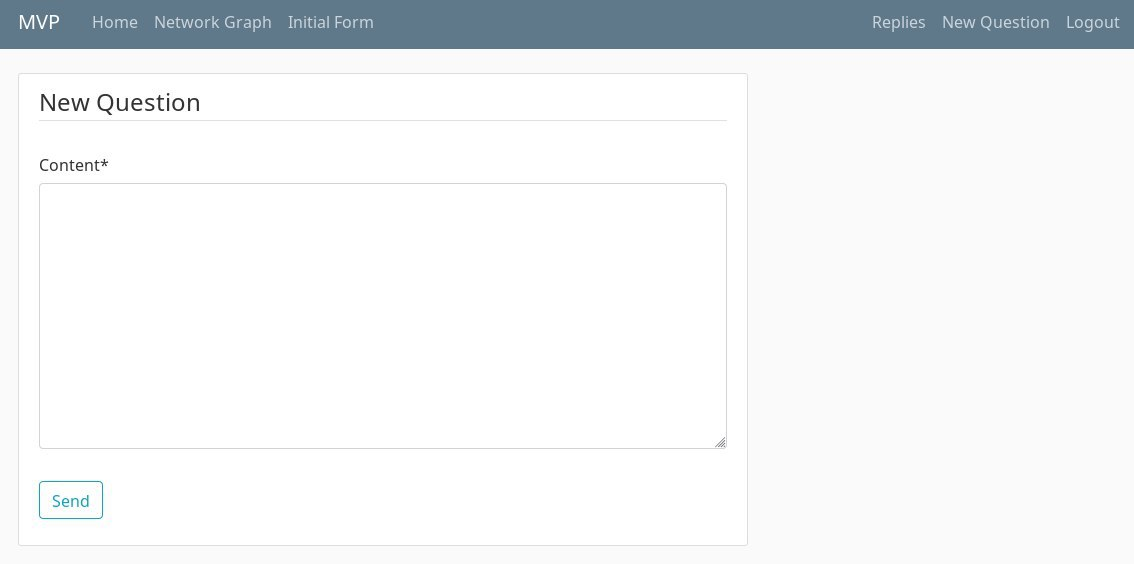
\includegraphics[width=14cm]{mvpCriarQuest.png}
\caption{Tela de criação de perguntas do MVP. Fonte: os autores.}
\label{fig:mvpCriarQuest}
\end{figure}

\begin{figure}[!htb]
\centering
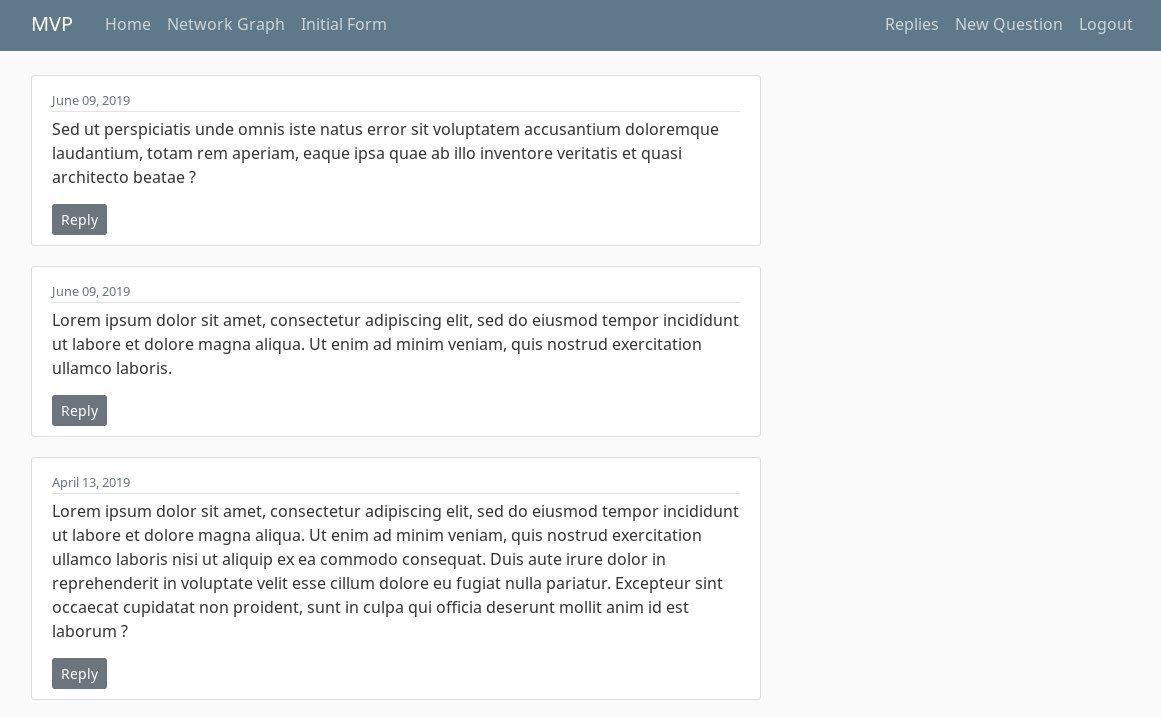
\includegraphics[width=14cm]{mvpVerQuest.png}
\caption{Tela de visualização de perguntas do MVP. Nesta tela é possível escolher uma pergunta para ser respondida. Fonte: os autores.}
\label{fig:mvpVerQuest}
\end{figure}

\begin{figure}[!htb]
\centering
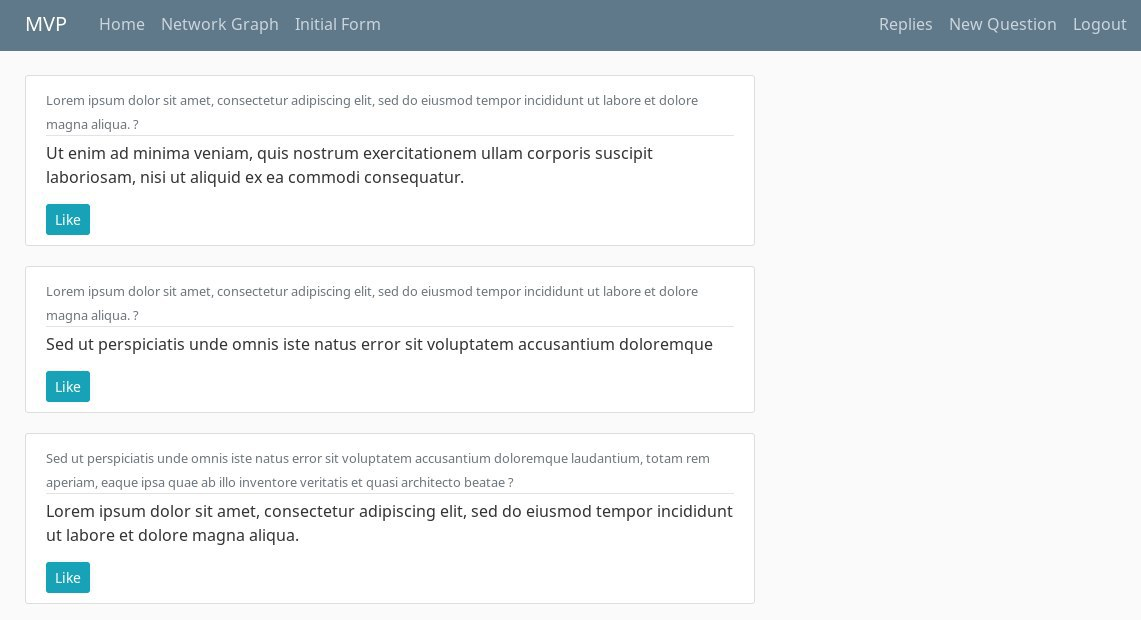
\includegraphics[width=14cm]{mvpVerResp.png}
\caption{Tela de visualização de respostas recebidas do MVP. Nesta tela é possível marcar perguntas favoritas. Fonte: os autores.}
\label{fig:mvpVerResp}
\end{figure}

\begin{figure}[!htb]
\centering
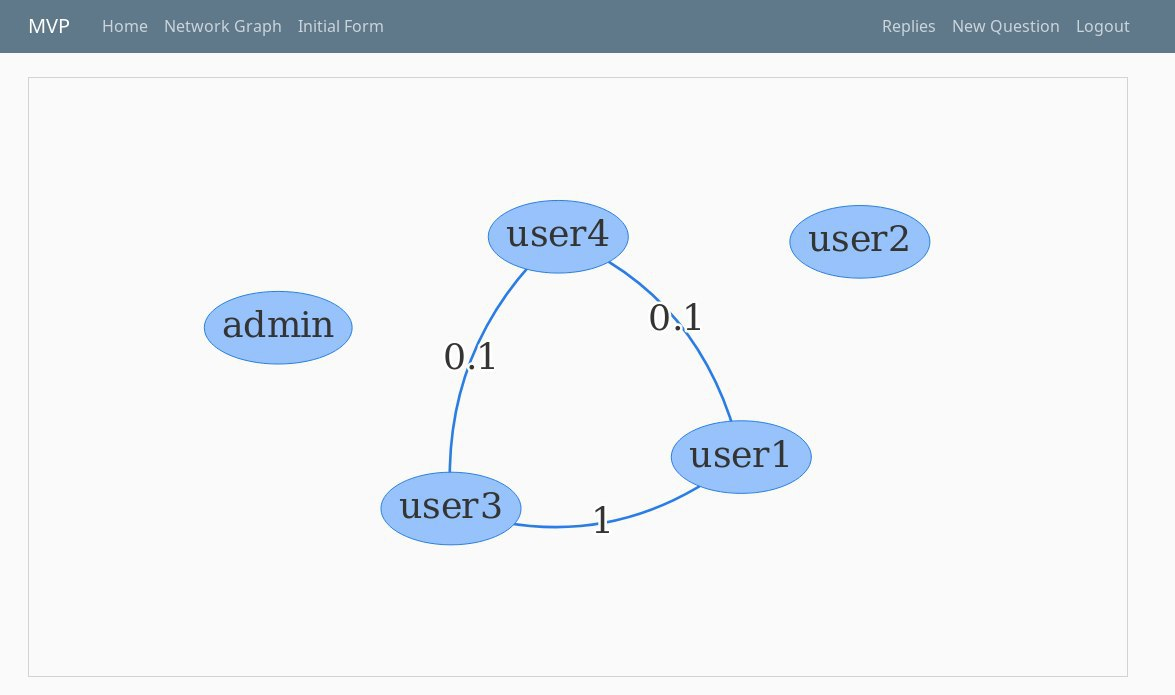
\includegraphics[width=14cm]{mvpVerGrafo.png}
\caption{Visualização do grafo que representa as ligações entre usuários da rede social no MVP. Fonte: os autores.}
\label{fig:mvpVerGrafo}
\end{figure}

\FloatBarrier


A figura \ref{fig:mvpVerGrafo} é a tela do MVP que representa os usuários e suas conexões criadas na rede social por meio de um grafo.


\section{Arquitetura}

\begin{itemize}
\item Qual a tecnologia
\item Custo
\item Arquitetura
\end{itemize}

Desenho da arquitetura

\begin{figure}[!htb]
\centering

\includegraphics[width=14cm]{arquitetura.png}
\caption{Arquitetura do software. Fonte: os autores.}
\label{fig:arquitetura}
\end{figure}

\FloatBarrier
%=====================================================

\section{Tecnologia aplicada}

\begin{itemize}
\item Linguagens de programação
\item Frameworks

\end{itemize}

Frameworks: IONIC django

angular e github.

Linguagens: python typescript javascript html/css
Hardware: PC Notebook thinkpad x201, SSD 120GB e 8GB de RAM primeira geracao do i5 e arch linux, server usa debian stretch
Infraestrutura: 	Docker
VPS: CPU: Intel (Haswell, noTSX) (1)@2.3GHz GPU: CirrusLogicGD5446 Memory: 583MB / 1956MB.



%=====================================================

\section{Análise do sistema}

Diagramas de caso de USO
\begin{figure}[!htb]
\centering
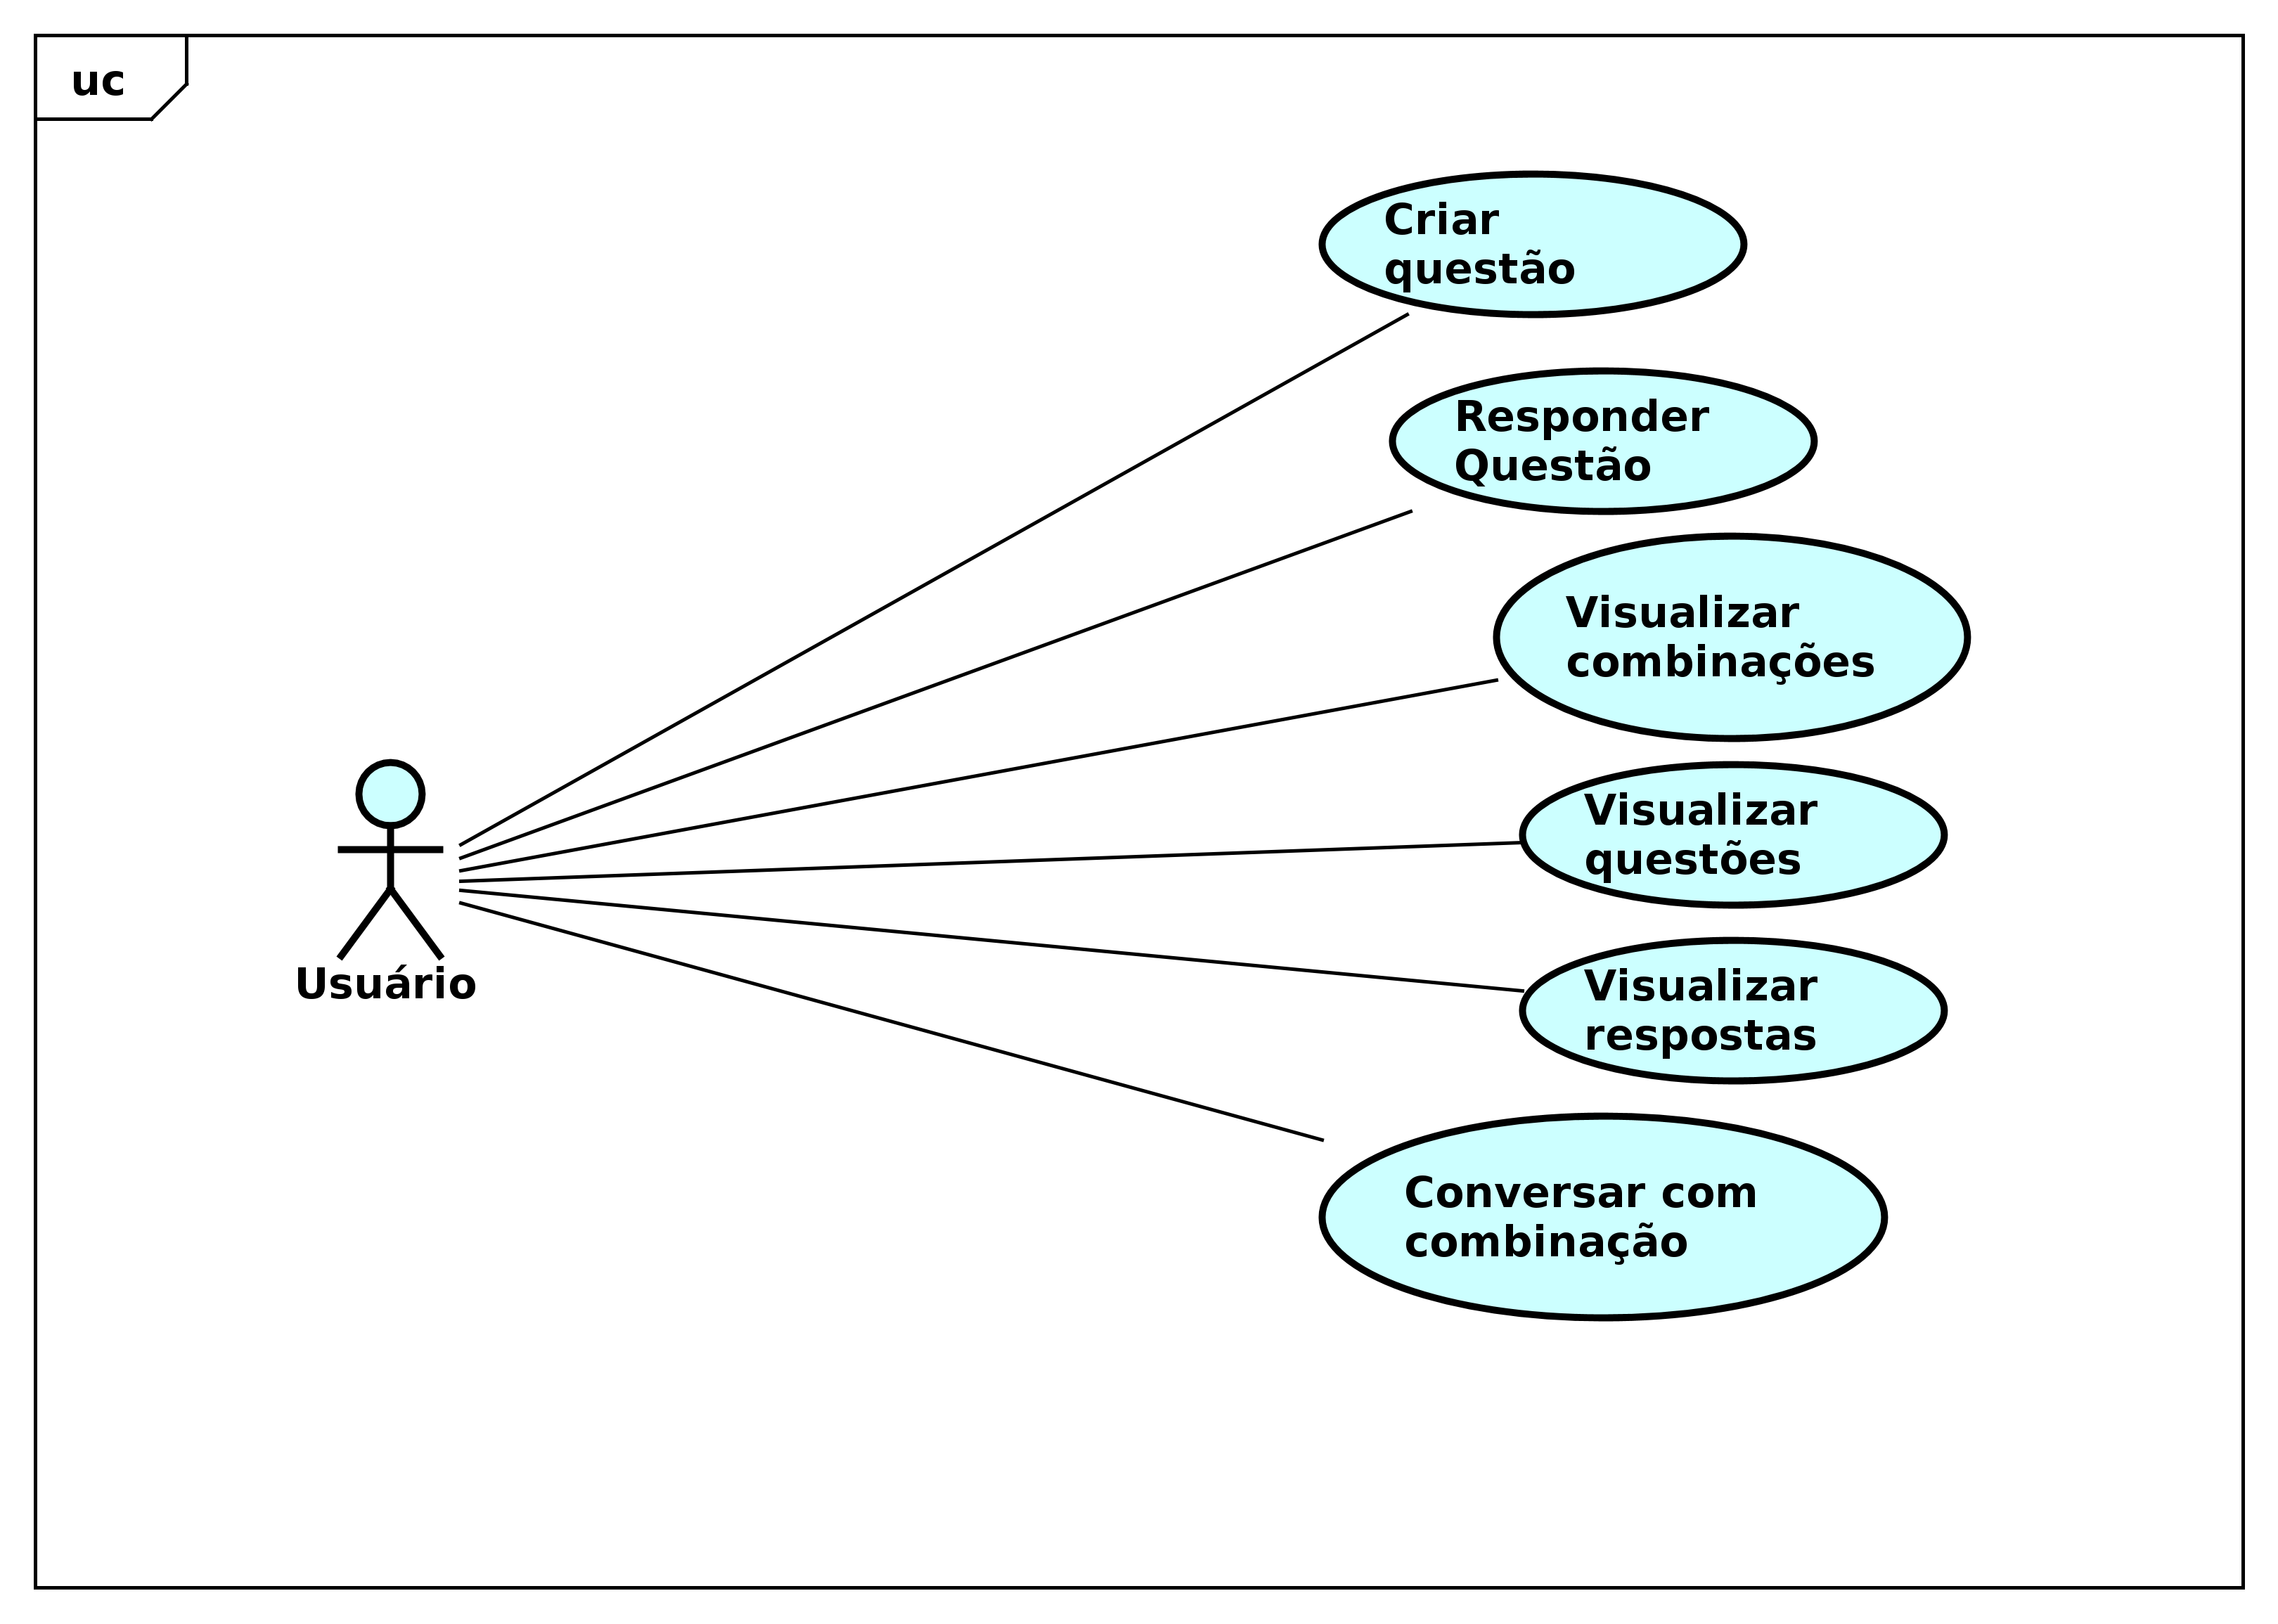
\includegraphics[width=16cm]{DCU1.png}
\caption{Diagrama de caso de uso nível 1. Fonte: os autores.}
\label{fig:DCU1}
\end{figure}

\begin{figure}[!htb]
\centering
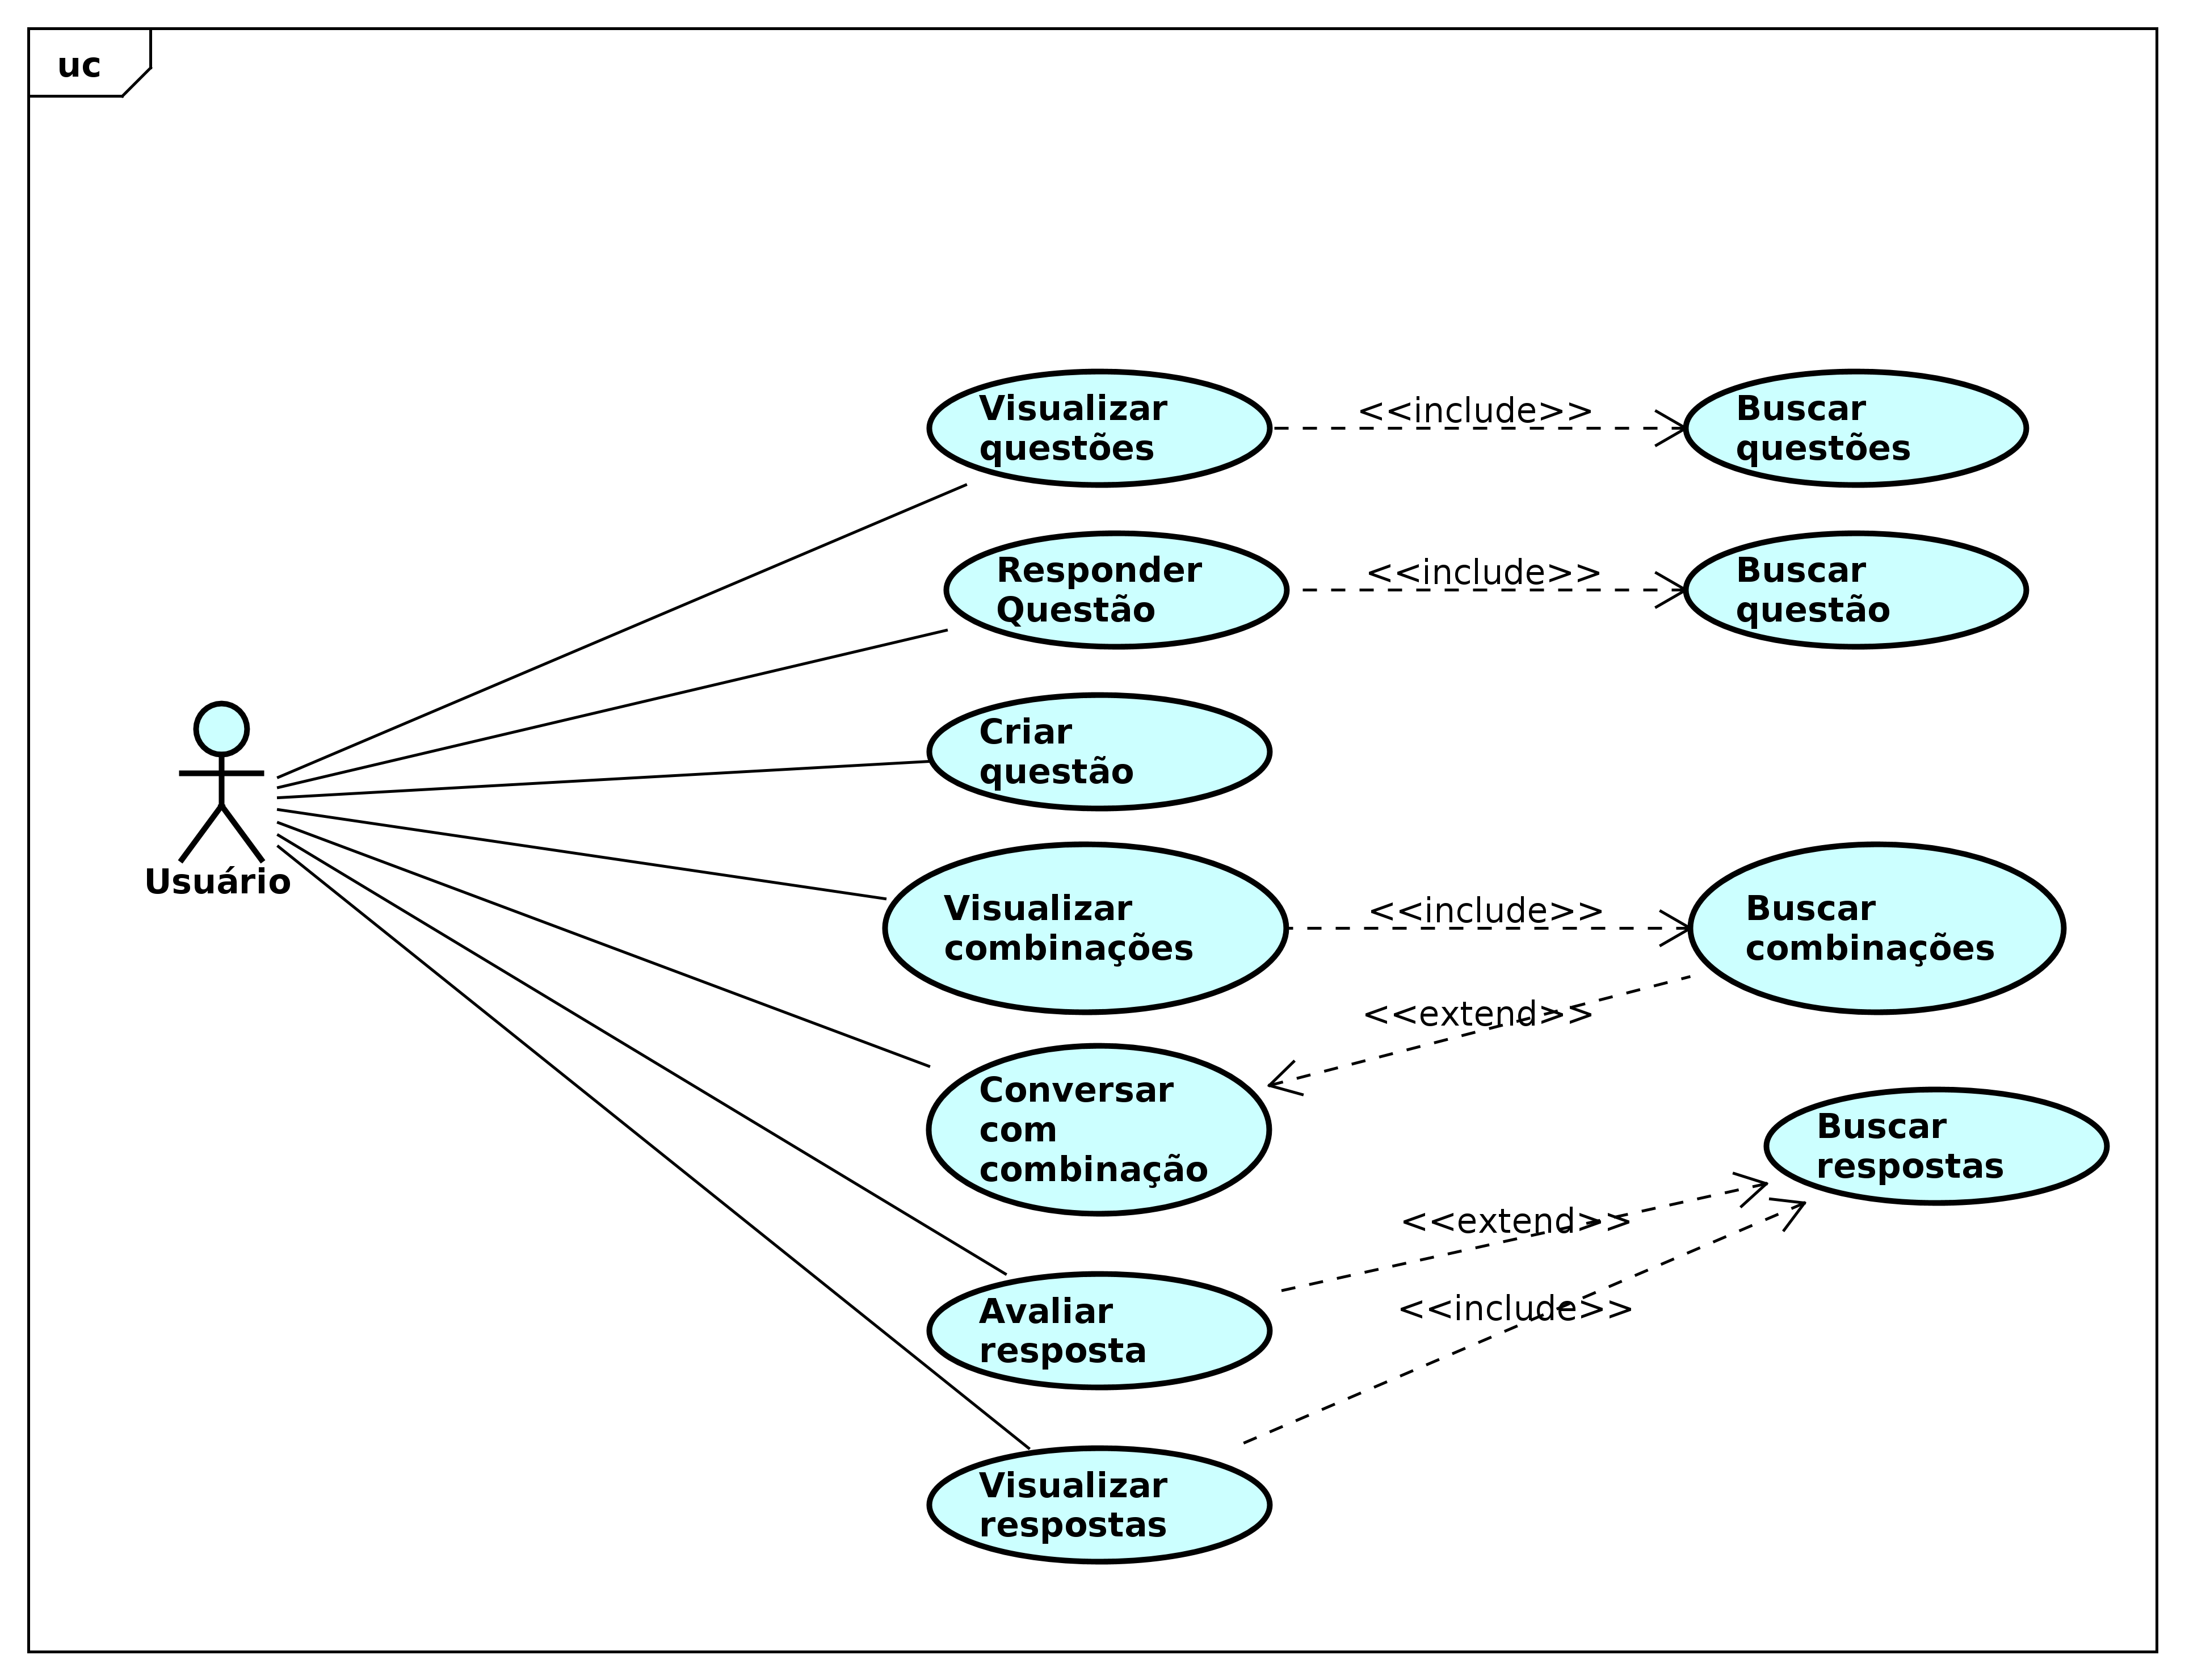
\includegraphics[width=16cm]{DCU2.png}
\caption{Diagrama de caso de uso nível 2. Fonte: os autores.}
\label{fig:DCU2}
\end{figure}
%=====================================================

Diagramas de sequência

\begin{figure}[!htb]
\centering
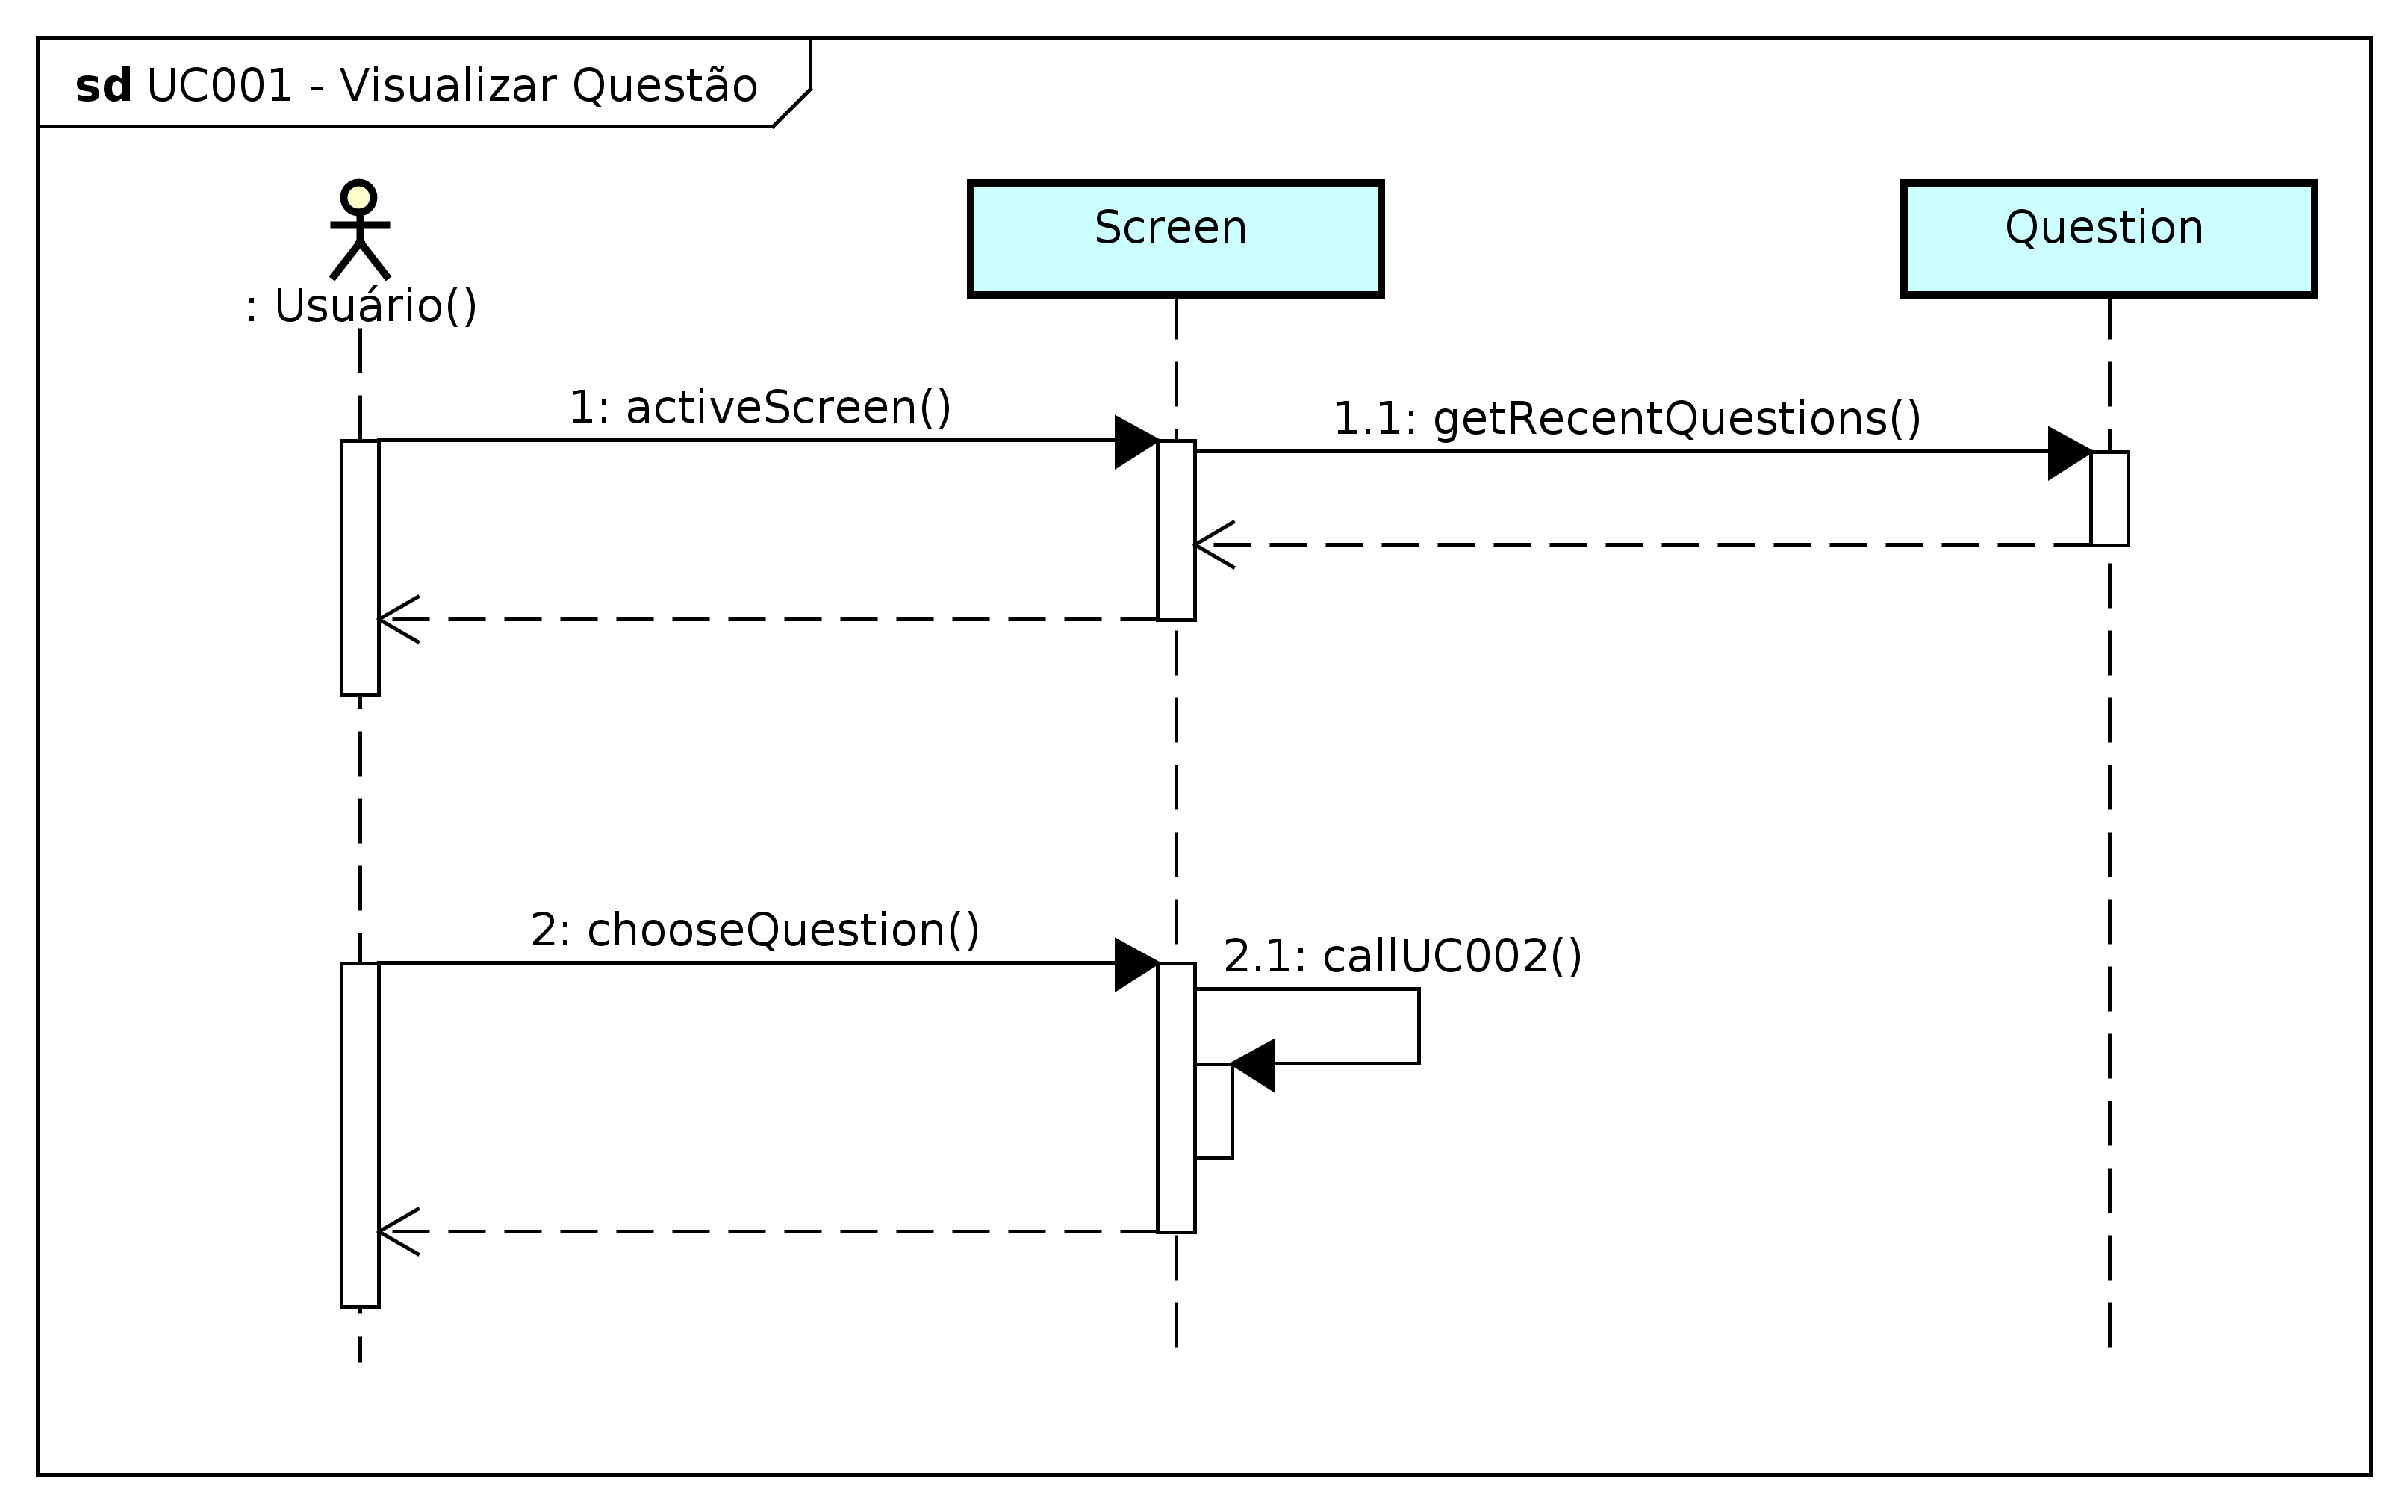
\includegraphics[width=16cm]{UC001-VisualizarQuestao.png}
\caption{Diagrama de caso de uso UC001 - Visualizar Questão. Fonte: os autores.}
\label{fig:UC001}
\end{figure}

\begin{figure}[!htb]
\centering
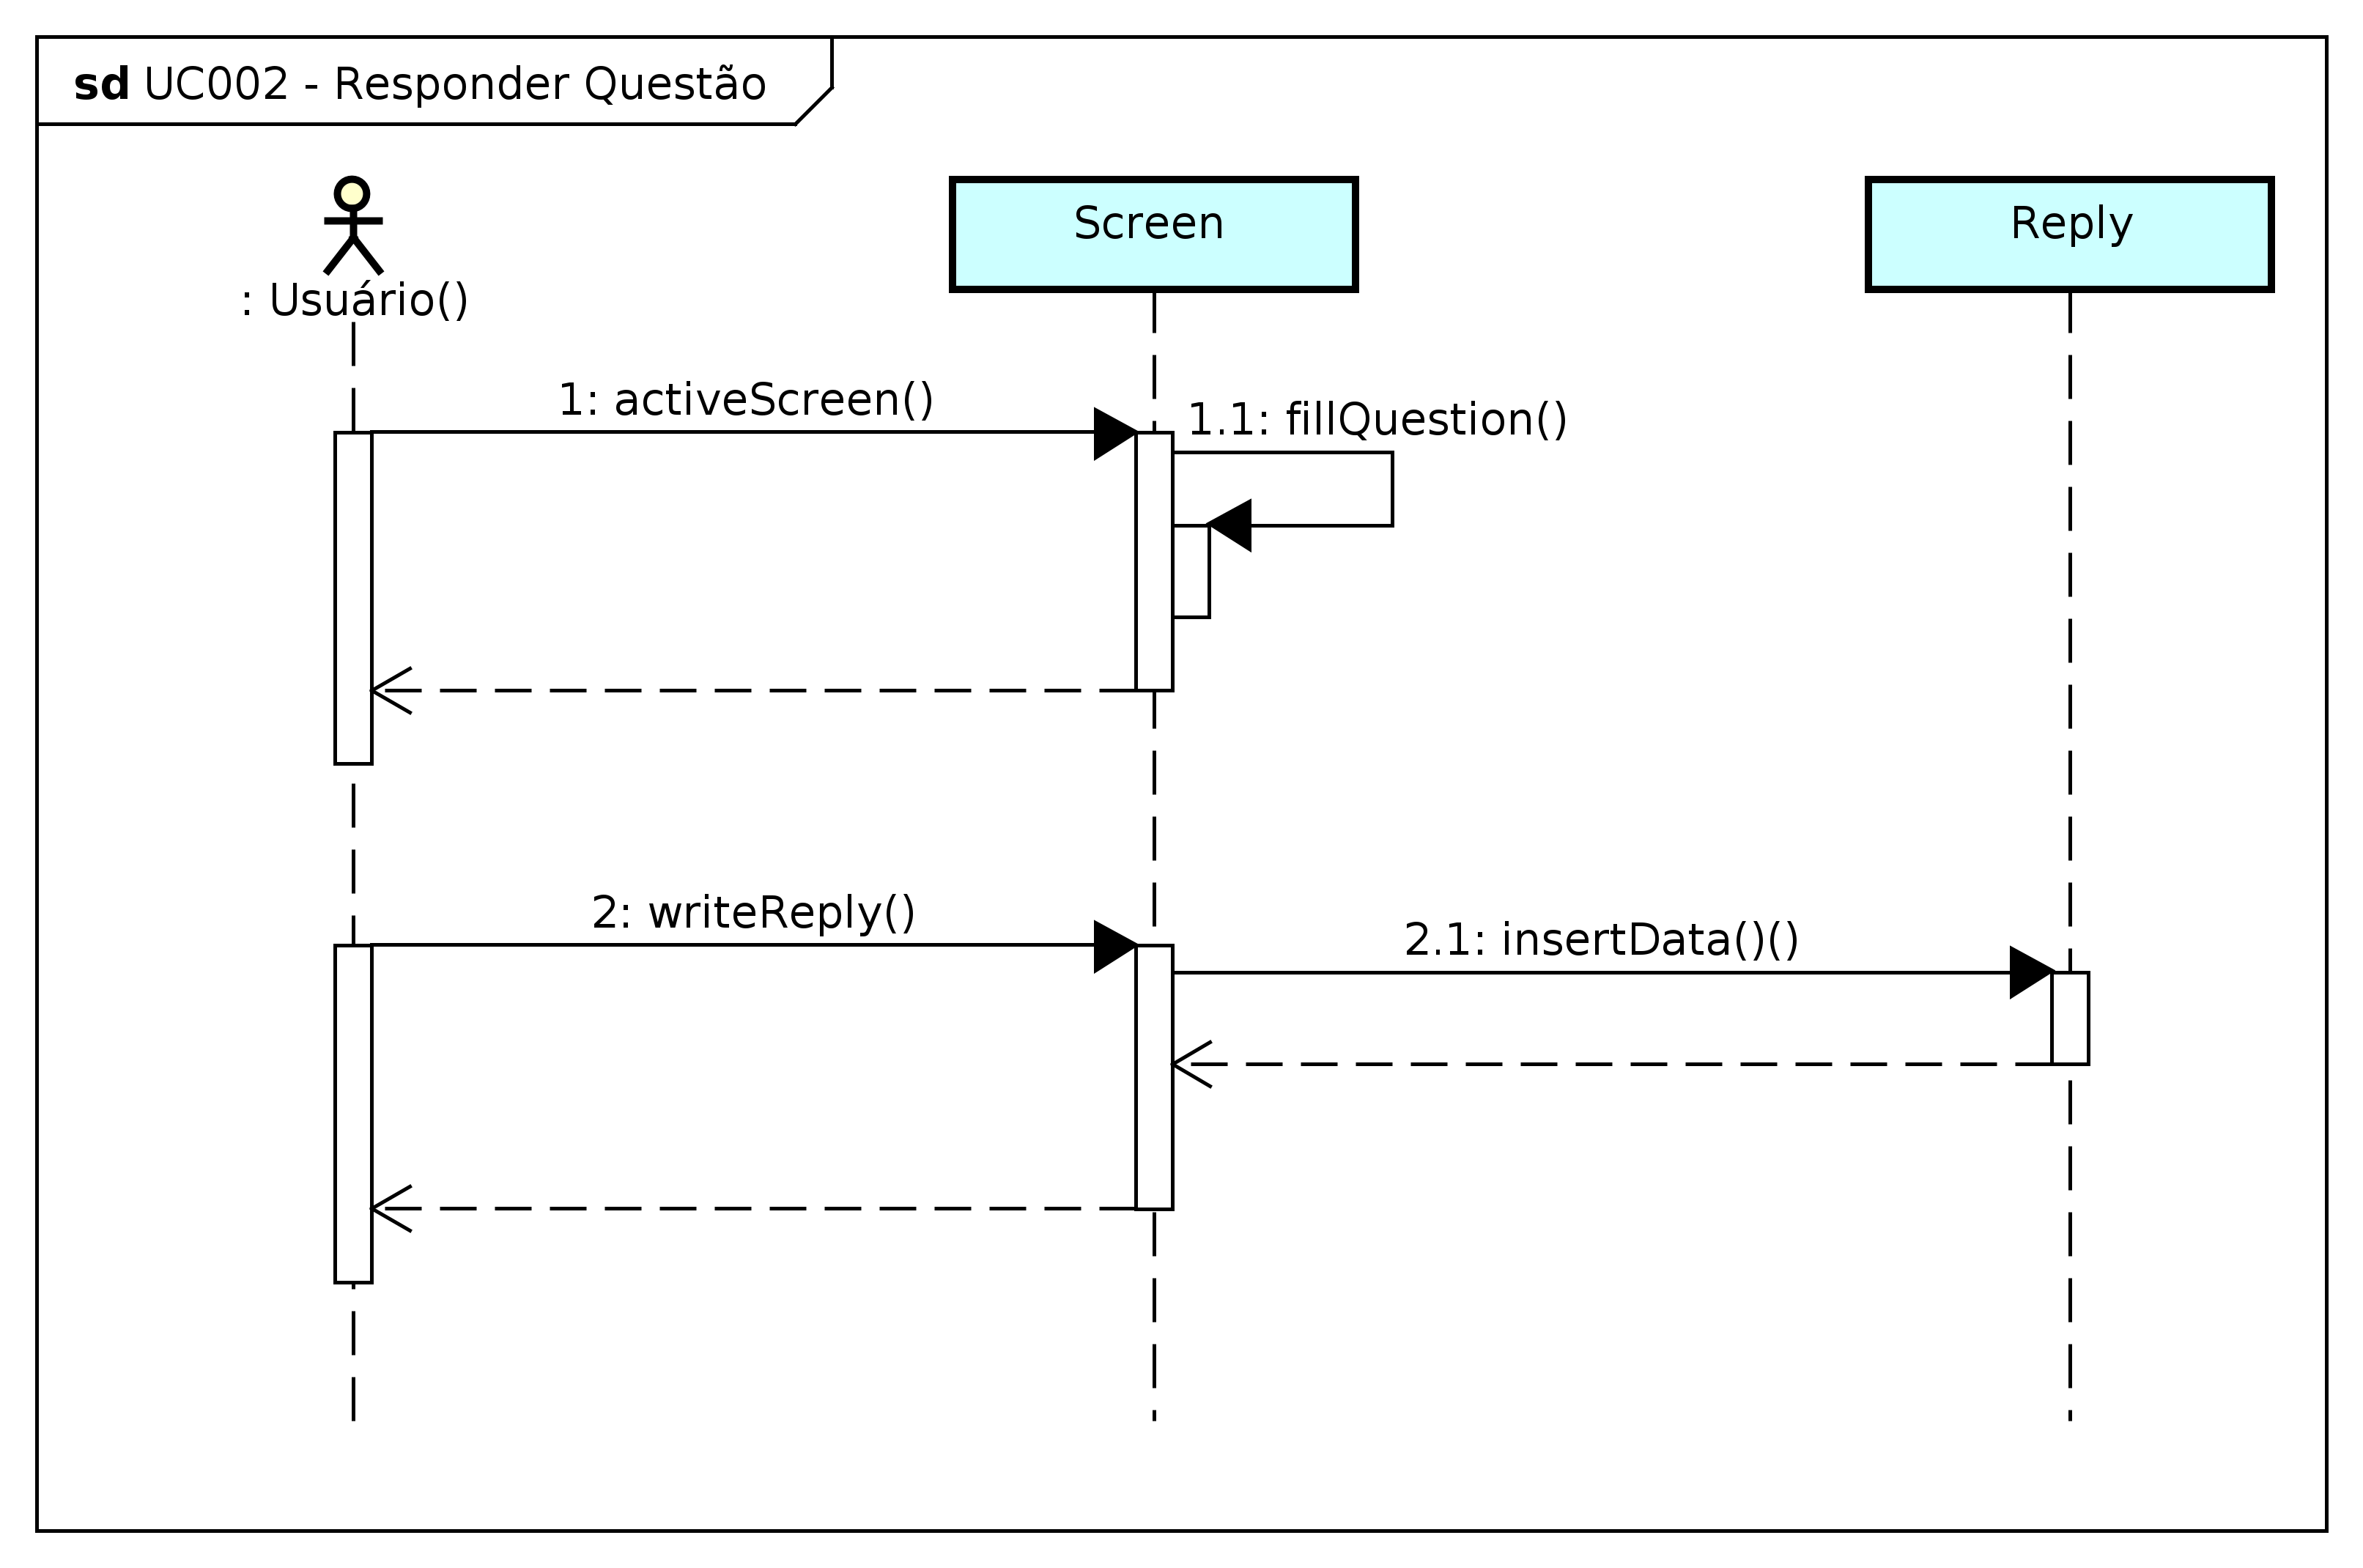
\includegraphics[width=16cm]{UC002-ResponderQuestao.png}
\caption{Diagrama de caso de uso UC002 - Responder Questão. Fonte: os autores.}
\label{fig:UC002}
\end{figure}

\begin{figure}[!htb]
\centering
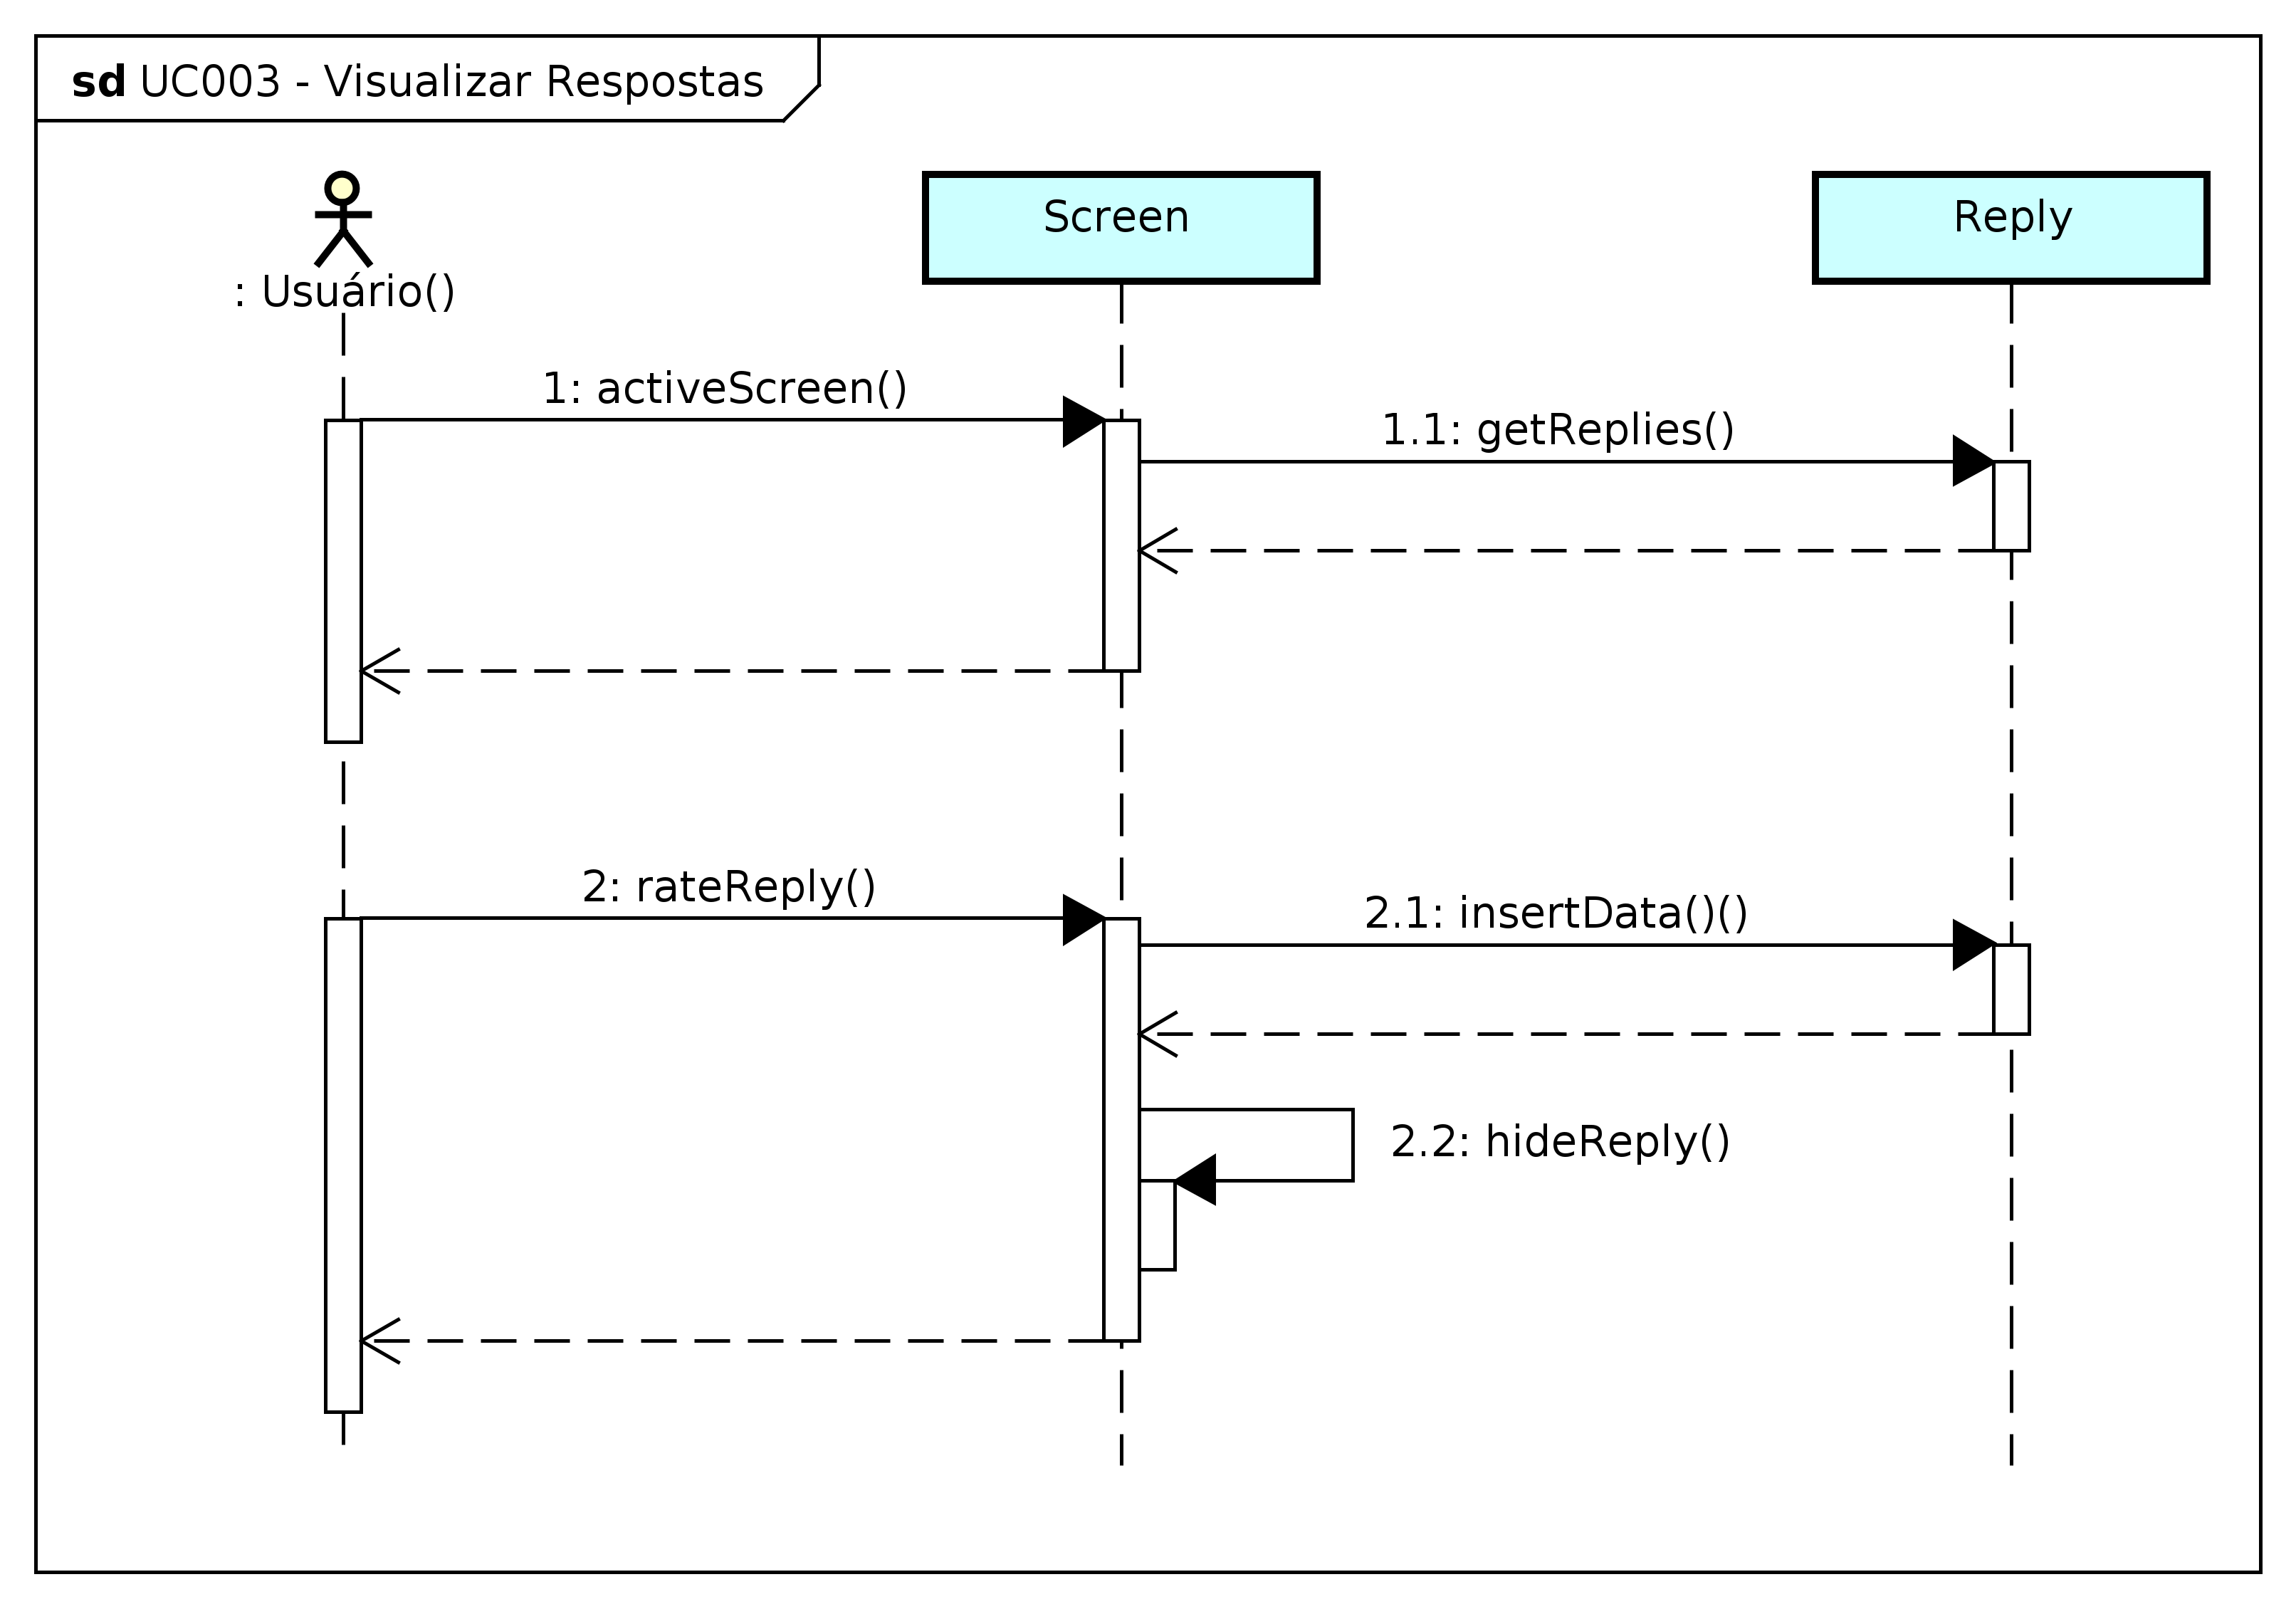
\includegraphics[width=16cm]{UC003-VisualizarRespostas.png}
\caption{Diagrama de caso de uso UC003 - Visualizar Respostas. Fonte: os autores.}
\label{fig:UC003}
\end{figure}


\begin{figure}[!htb]
\centering
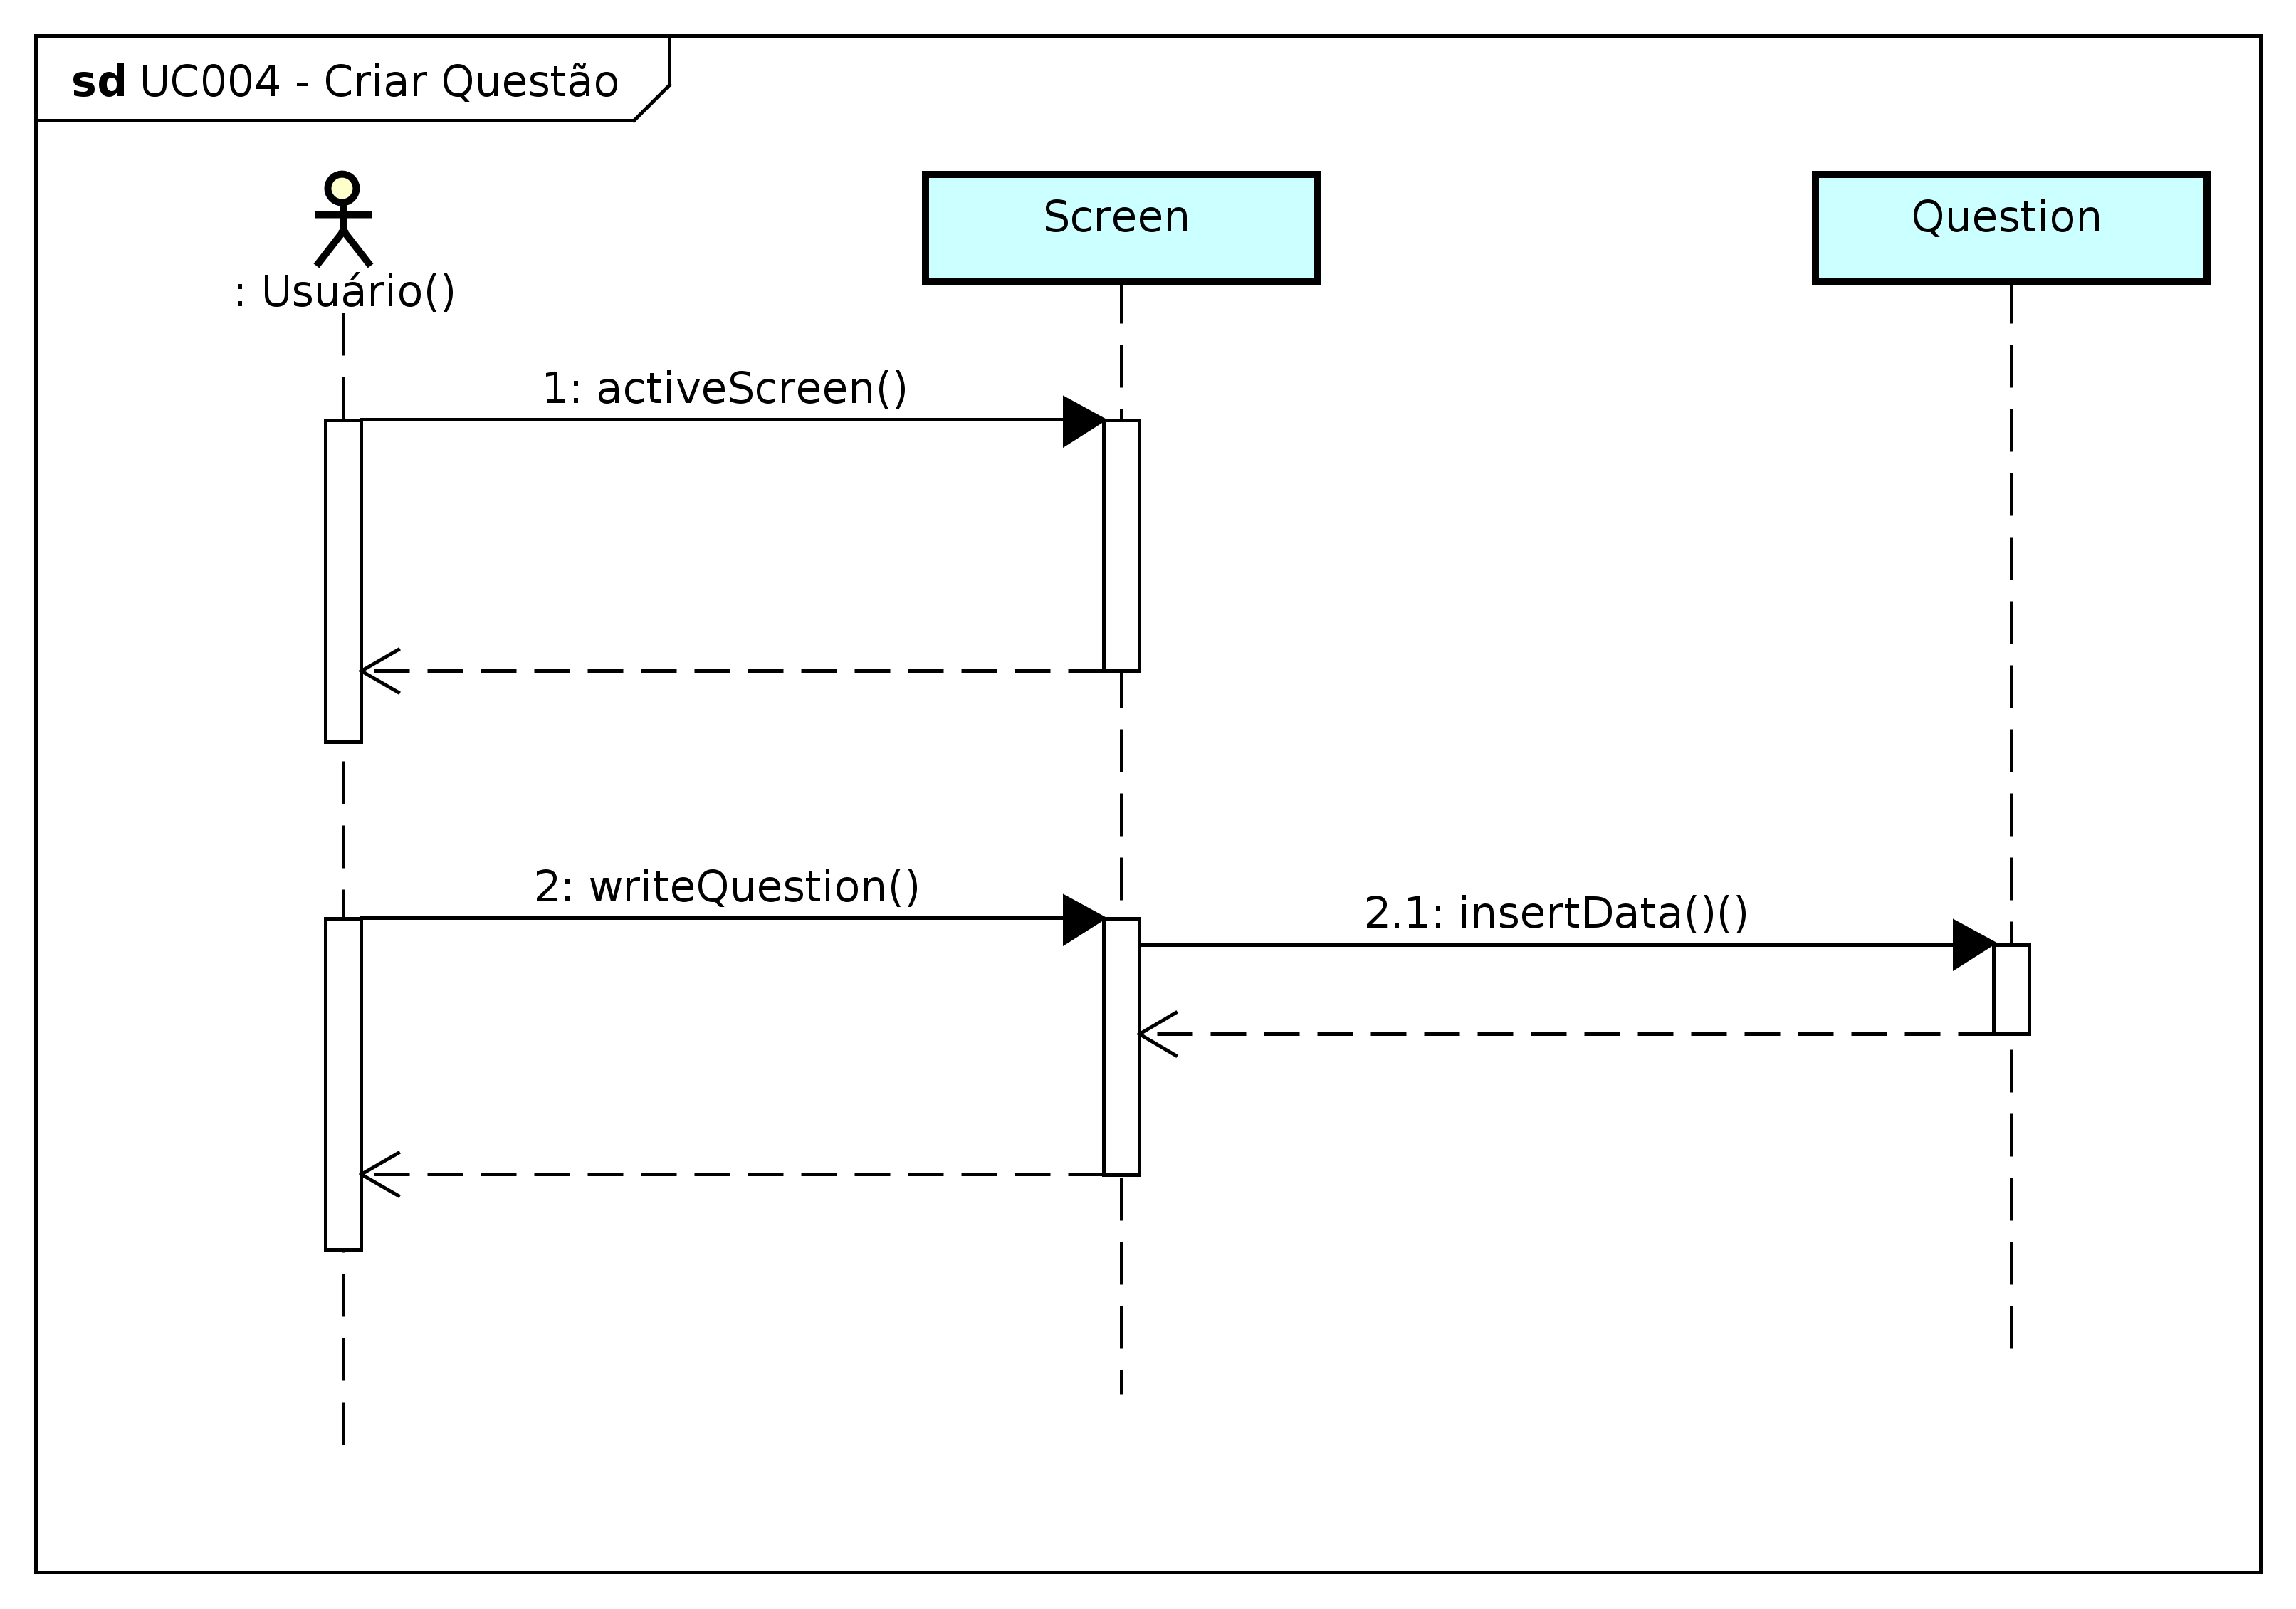
\includegraphics[width=16cm]{UC004-CriarQuestao.png}
\caption{Diagrama de caso de uso UC004 - Criar Questão. Fonte: os autores.}
\label{fig:UC004}
\end{figure}


\begin{figure}[!htb]
\centering
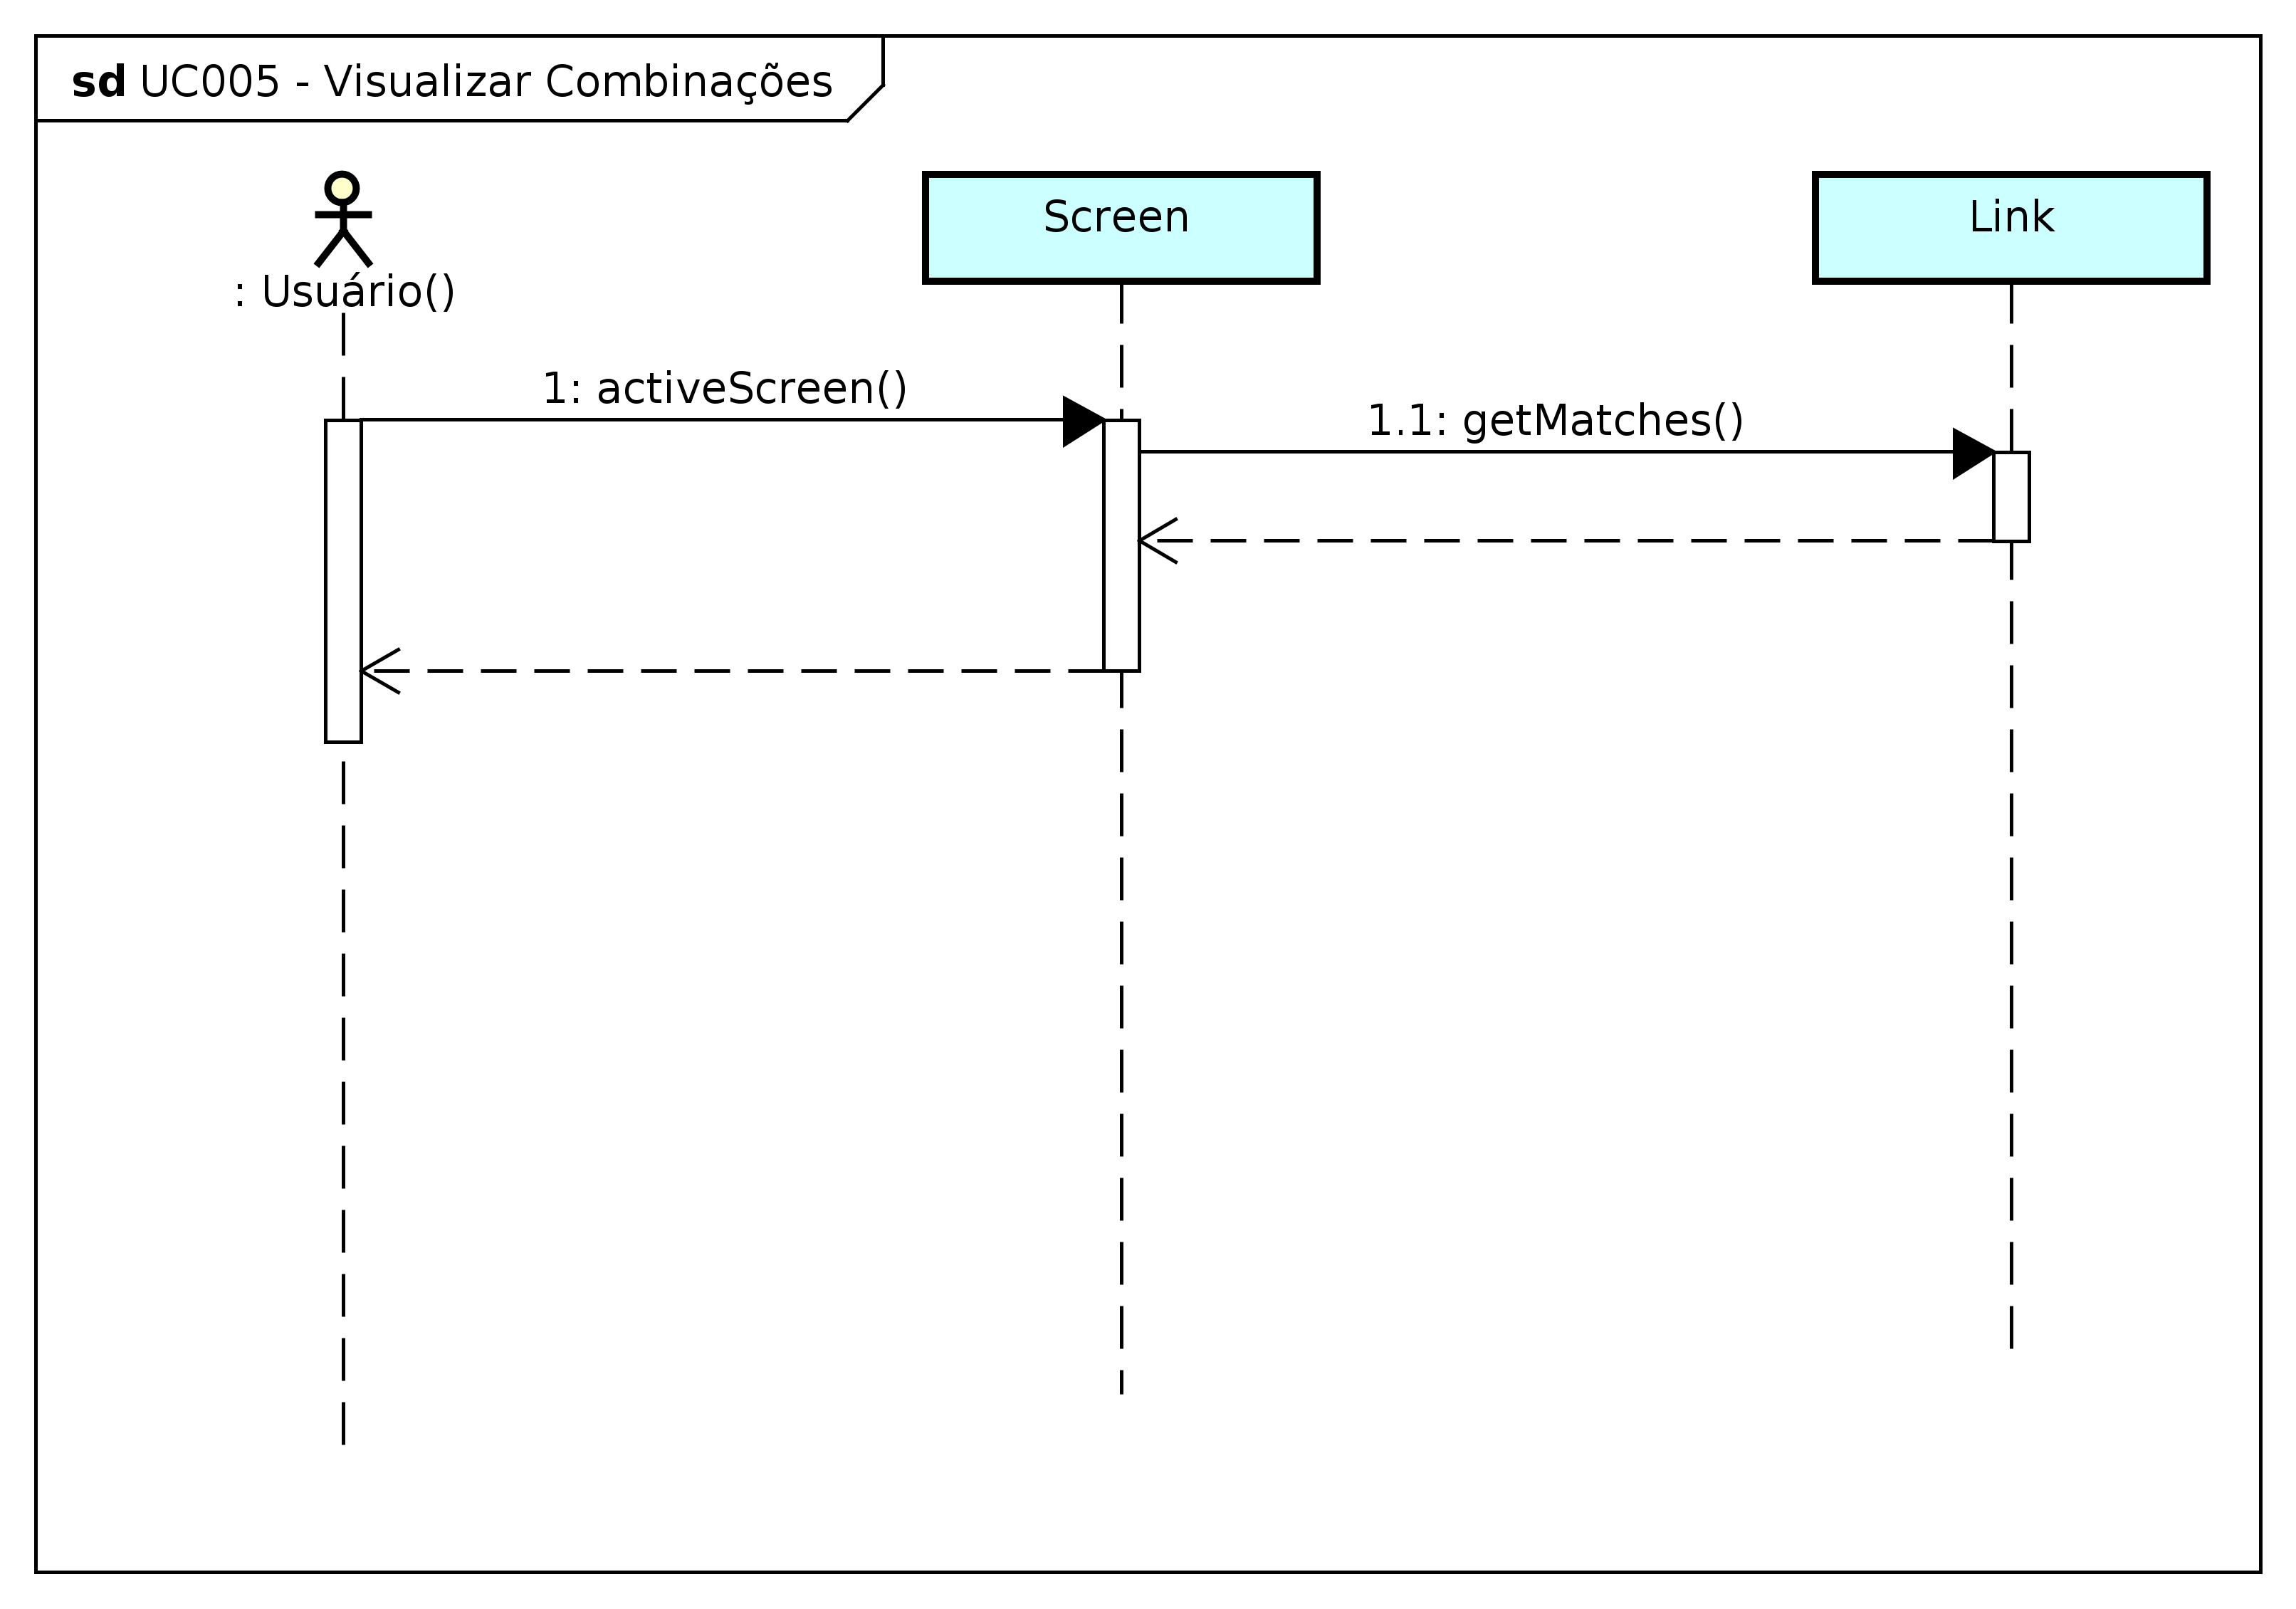
\includegraphics[width=16cm]{UC005-VisualizarCombinacoes.png}
\caption{Diagrama de caso de uso UC005 - Visualizar Combinações. Fonte: os autores.}
\label{fig:UC005}
\end{figure}


Diagrama de Classes

\begin{figure}[!htb]
\centering
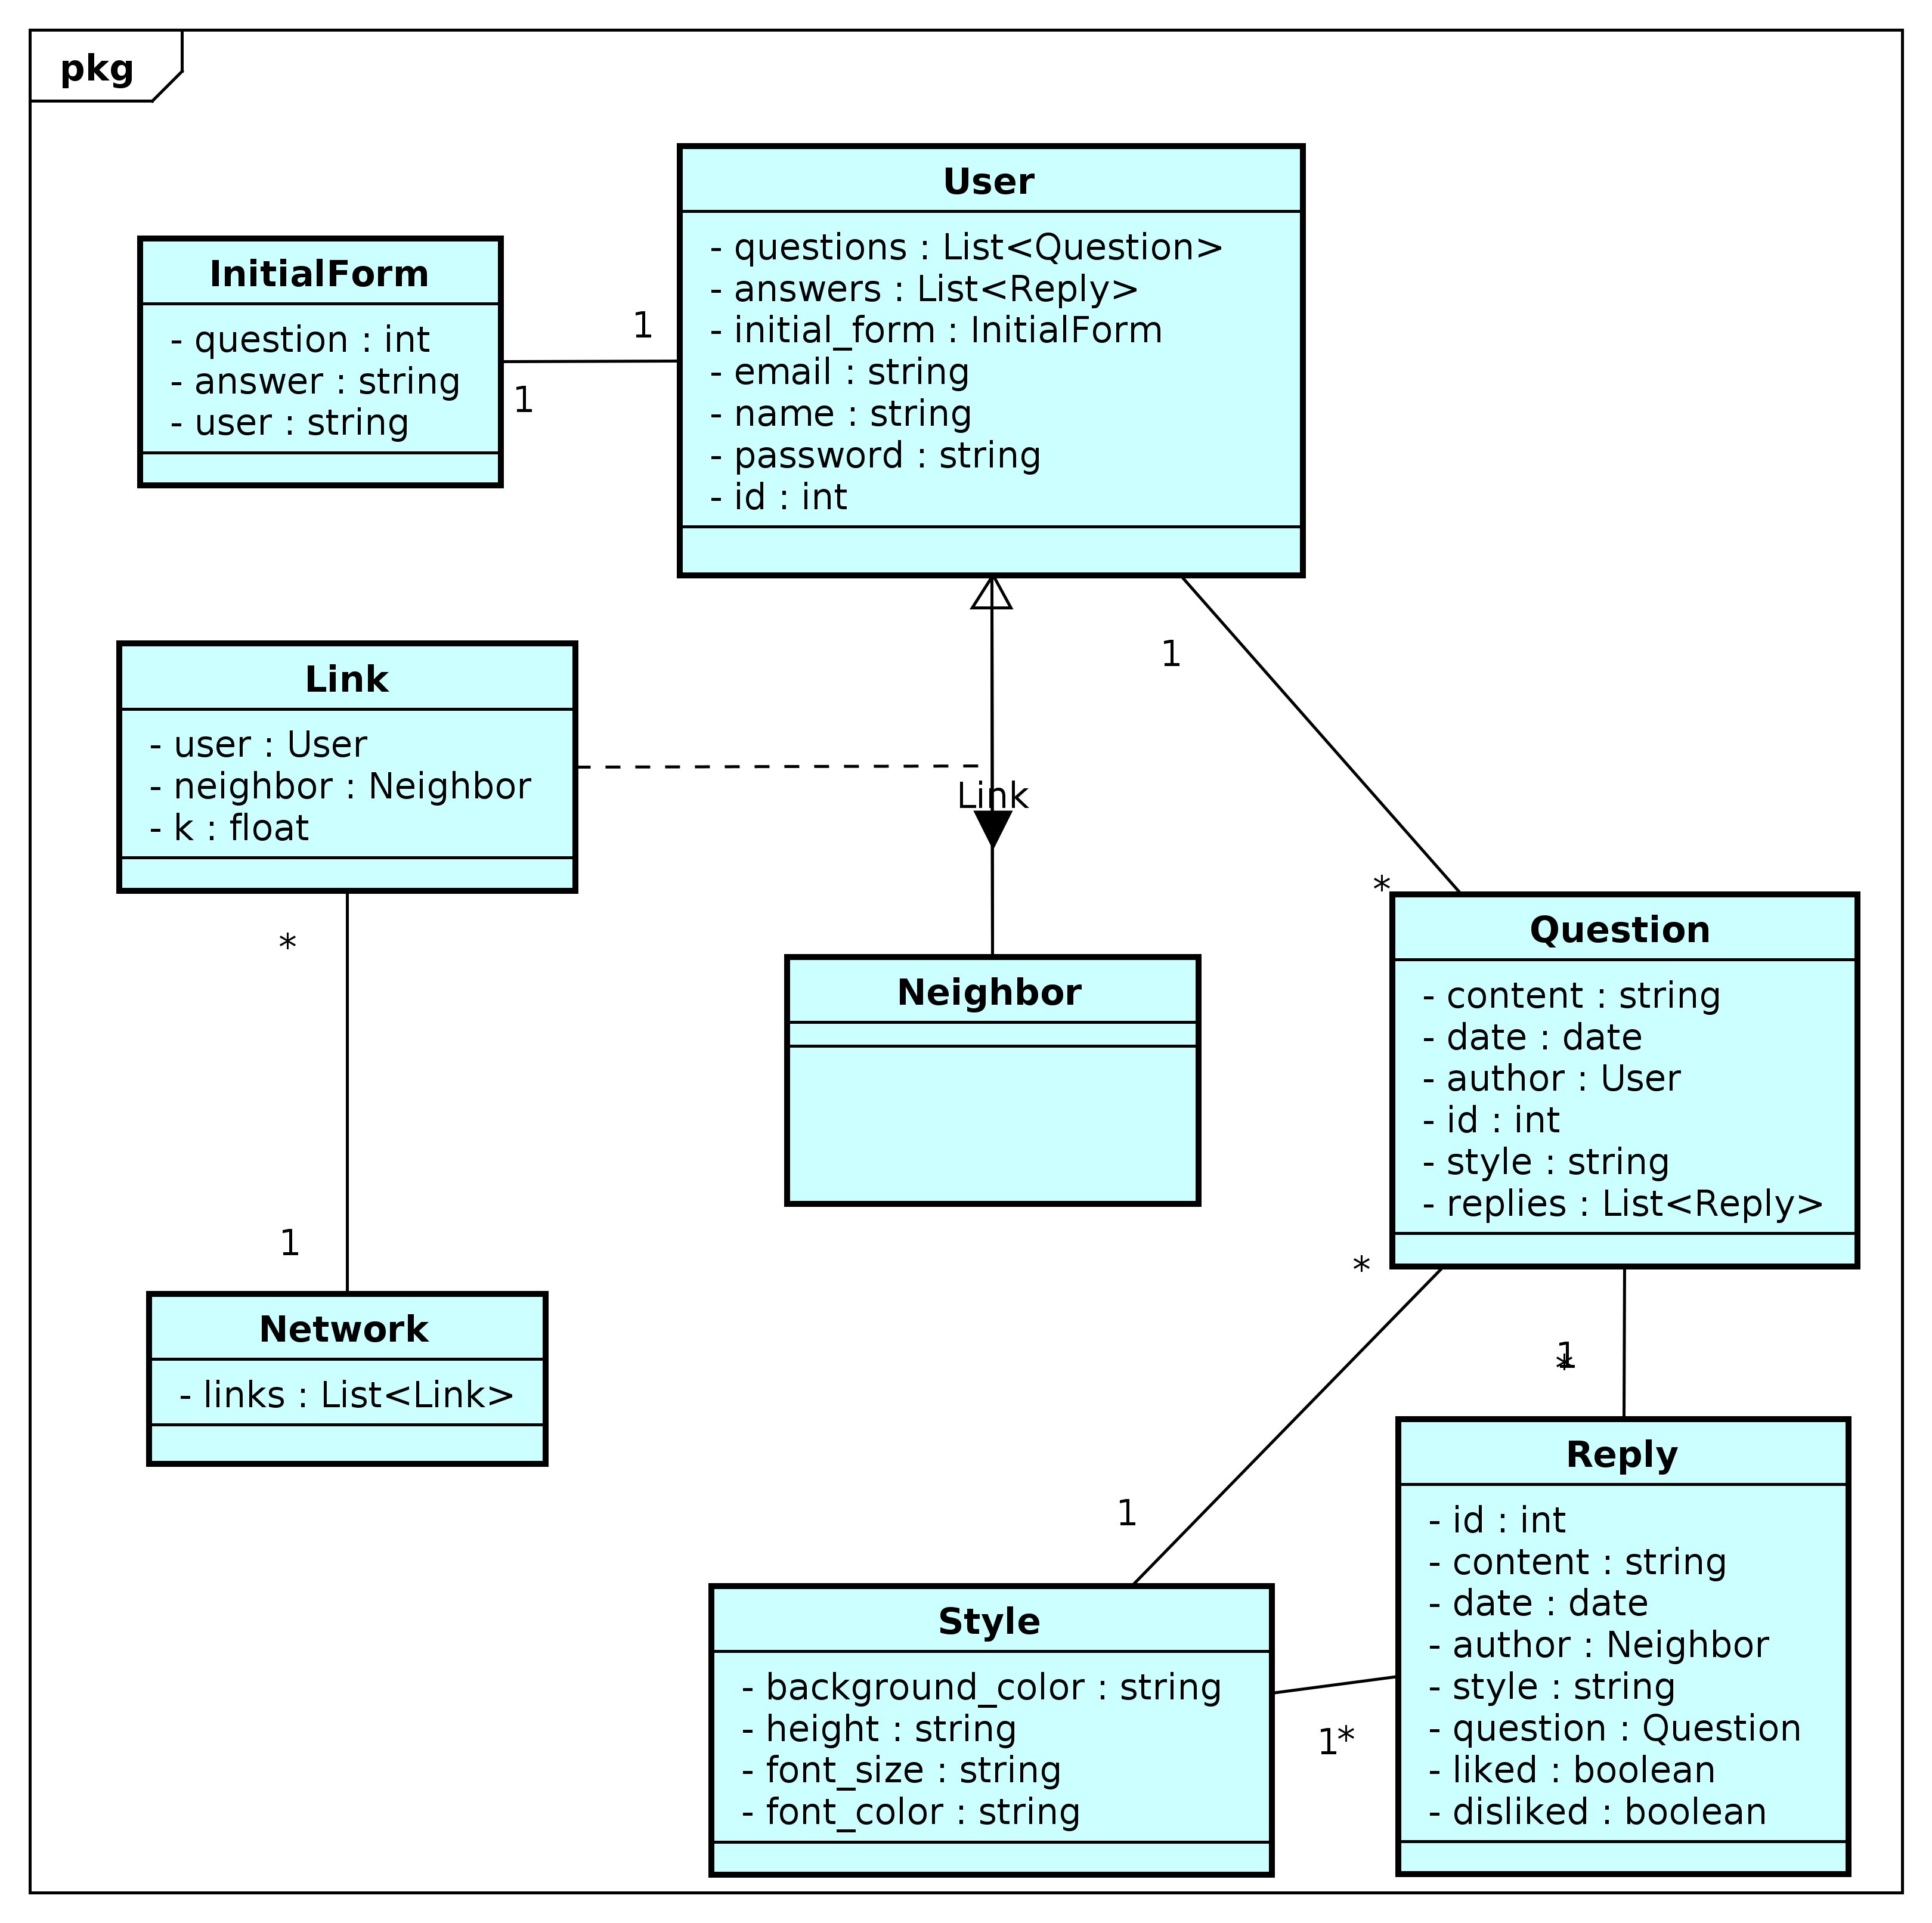
\includegraphics[width=16cm]{DiagramaClasse.png}
\caption{Diagrama de classes. Fonte: os autores.}
\label{fig:diagramaClasse}
\end{figure}
\FloatBarrier



%=====================================================

\section{Cálculo de do peso da aresta}
O peso de uma aresta do grafo, $k$, representa o nível de afinidade entre os dois usuários conectados por esta aresta. Um usuário pode estar conectado a vários outros usuários.

Quando um usuário entra pela primeira vez na rede social, ele é obrigado a preencher um questionário contendo as questões constantes na tabela \ref{tab:questoes}. A partir das respostas deste questionário, um valor para $k$ é calculado levando em conta, tão somente, a similaridade entre as respostas de cada usuário.

\begin{table}[!htp]
\centering
\caption{Formulário inicial}
\label{tab:questoes}
\begin{tabular}{ || c ||}
\hline
Pergunta\\
\hline
\hline
Você prefere cachorro ou gato?\\  
\hline
Você prefere rock ou funk?\\
\hline
Você prefere verão ou inverno? \\
\hline
Você prefere cinema ou teatro?\\
\hline
Você prefere cerveja ou vinho?\\
\hline
Você prefere o dia ou a noite?\\
\hline
Você prefere sair ou ficar em casa?\\
\hline
Você fuma?\\
\hline
Você tem alguma religião?\\
\hline
Você acredita em signos?\\
\hline
Você prefere praia ou campo?\\
\hline
\end{tabular}
\end{table}

Para a determinação inicial de $k$, logo após o preenchimento do formulário, é calculado o total de respostas iguais entre dois usuários e aplicada a seguinte equação:

\begin{equation}
k_{ab} = \frac{R_{ab}*(x-1)}{N_{p}}
 \label{eq:k0}
\end{equation}


Onde $R_{ab}$ é o total de respostas do usuário A iguais ao usuário B; $x$ é o valor objetivo para considerar dois usuários similares - este valor será discutido adiante nesta seção - e $N_{p}$ é o total de perguntas do questionário inicial.

Na equação \ref{eq:k0}, o numerador é multiplicado por $x-1$ para que os usuários que tiveram todas as questões respondidas da mesma maneira no questionário tão somente fiquem muito próximos da margem que define a habilitação do mensageiro instantâneo. O objetivo é tornar obrigatória a interação por meio de perguntas e respostas antes que dois usuários possam ser considerados similares o suficiente para desfrutarem do mensageiro.

Então, conforme as perguntas postadas pelos usuários vão sendo respondidas e apreciadas, valor do peso da aresta, definido como $k_{ab}$, que liga os usuários $A$ e $B$, é recalculado, para cada resposta apontada como apreciada, a partir da seguinte definição:

\begin{equation}
k_{ab} = k_{ab} + \frac{(R_{ab} + R_{ba})}{(P_{A} + P_{B})}
\label{eq:k1}
\end{equation}

Onde $R_{ab}$ é o número de respostas que o usuário $A$ recebeu do usuário $B$ e $A$ gostou; $R_{ba}$ é o número de respostas que o usuário $B$ recebeu do usuário $A$ e a $B$ gostou; $P_{A}$ é o número de perguntas postadas pelo usuário $A$ e $P_{B}$ o número de respostas postadas pelo usuário $B$.

Na figura \ref{fig:grafico_k1}, podemos ver a evolução do peso $k$ para cada resposta recebida pelo usuário $A$ que ele gostou. Nesta situação o crescimento do valor de $k$ é linear, pois todas as perguntas postadas pelo usuário $A$ estão respondidas por $B$ e as respectivas respostas foram curtidas.

\begin{figure}[!htb]
\centering
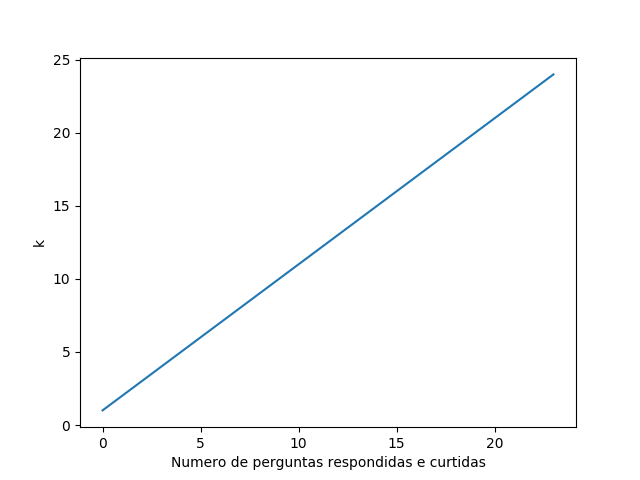
\includegraphics[width=14cm]{grafico_k1.png}
\caption{Evolução de $k$ se todas as perguntas postadas por $A$ forem respondidas por $B$. Fonte: os autores.}
\label{fig:grafico_k1}
\end{figure}

Como o cálculo leva em conta todas as perguntas postadas pelo usuário $A$, no caso de já haver perguntas postadas e não respondidas, o crescimento do valor de $k$ é afetado num grau inversamente proporcional ao número de perguntas postadas, como pode-se observar na figura \ref{fig:grafico_k2}.

\begin{figure}[!htb]
\centering
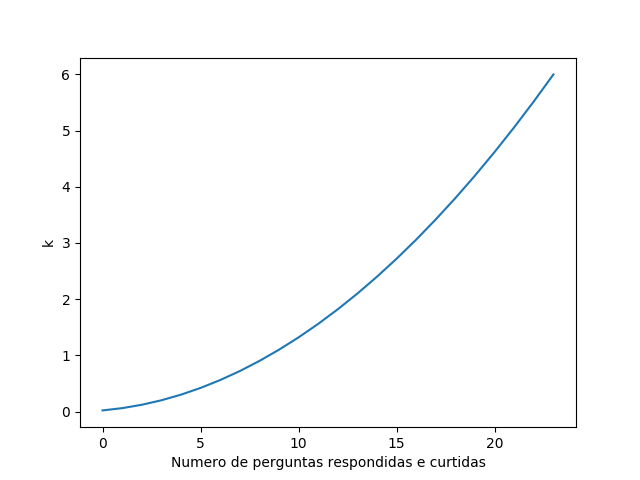
\includegraphics[width=14cm]{grafico_k2.png}
\caption{Evolução de $k$ se $A$ postou 50 perguntas e apenas 25 respostas de $B$ foram curtidas. Fonte: os autores.}
\label{fig:grafico_k2}
\end{figure}

É importante observar que o peso do incremento para $k$ é menor quando maior for o número de perguntas postadas seja por $A$ ou $B$. Dessa maneira, podemos depreender que a interação entre usuários novos, ou com poucas perguntas postadas, terá influência maior no crescimento do valor de $k$. Por outro lado, a interação entre usuários com muitas perguntas já postadas, incrementará um valor menor sobre $k$.

Tendo calculado um peso para cada aresta que liga os usuários, foi necessário definir um limiar $x$ que seria o valor mínimo de $k$ para considerar que dois usuários são similares o suficiente para serem postos em contato sob o mensageiro instantâneo.

A definição de $x$ provou-se um desafio, tendo em vista que o comportamento de $k$ varia em função do número total de perguntas postadas por dois usuários em análise. A figura \ref{fig:poucasquestoes} mostra que a convergência para $x = 1$ para o caso de de dois usuários que postaram poucas perguntas é rápida, pois o incremento de $k$ é maior. No caso simulado na figura \ref{fig:poucasquestões}, pouco mais de cinco respostas curtidas foram o suficiente para atingir o $x$.

\begin{figure}[!htb]
\centering
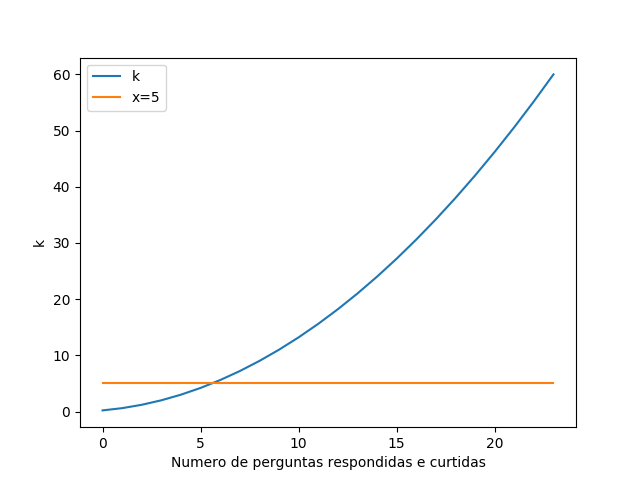
\includegraphics[width=14cm]{poucasquestoes.png}
\caption{Evolução de $k$ em função das respostas curtidas se $A$ e $B$ têm poucas perguntas postadas. Ex.: menos que 10 perguntas. Fonte: os autores.}
\label{fig:poucasquestoes}
\end{figure}

A figura \ref{fig:muitasquestoes}  demonstra que a convergência de $k$ e $x$ para usuários que já postaram muitas perguntas demanda muito mais respostas curtidas, neste caso mais que vinte respostas. Isto deve-se ao fato de ter sido decidido que a equação \ref{eq:k1} tem como divisor a soma de todas as perguntas já postadas pelos dois usuários, portanto, o incremento de $k$ é inversamente proporcional à soma de todas as perguntas postadas pelos usuários. 

\begin{figure}[!htb]
\centering
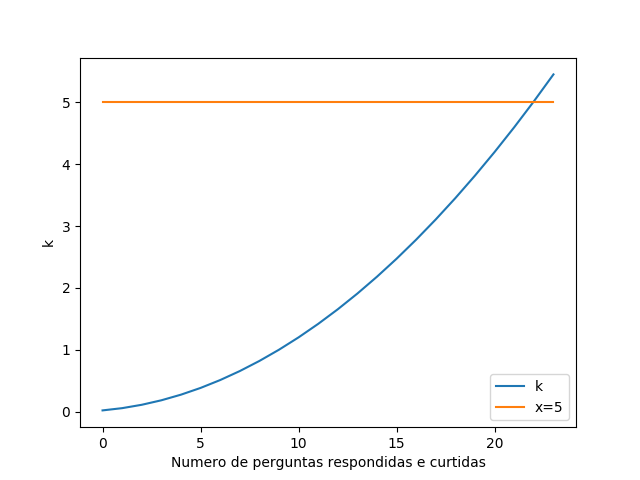
\includegraphics[width=14cm]{muitasquestoes.png}
\caption{Evolução de $k$ em função das respostas curtidas se $A$ e $B$ têm muitas perguntas postadas. Ex.: mais que 50 perguntas. Fonte: os autores.}
\label{fig:muitasquestoes}
\end{figure}

Uma adequação simplista para este problema seria definir $k$ como o número total de respostas curtidas entre dois usuários. Assim, $x$ seria o número mínimo de respostas que teriam que ser curtidas entre os usuários para que fossem considerados similares o suficiente para contatarem-se pelo mensageiro instantâneo. Porém, dessa maneira ignora-se que, se houverem muitas perguntas postadas por $A$ sem resposta de $B$ é possível que hajam mais diferenças do que similaridades entre os usuários, haja vista que muitas perguntas são ignoradas.

Portanto, é imprescindível considerar o volume de perguntas postadas. Uma evolução poderia adequar o software para contabilizar o número de perguntas postadas por $A$ e \emph{vistas} por $B$. Assim, poderíamos adequar o cálculo de $k$ como segue: 

\begin{equation}
k = k + \frac{R_{ab} + R_{ba}}{P_{AvB} + P_{BvA}} 
\label{eq:k2}
\end{equation}

Onde $R_{ab}$ é o número de respostas que o usuário $A$ recebeu do usuário $B$ e $A$ gostou; $R_{ba}$ é o número de respostas que o usuário $B$ recebeu do usuário $A$ e a $B$ gostou; $P_{AvB}$ é o número de perguntas postadas pelo usuário $A$ e vistas por $B$ e $P_{BvA}$ o número de respostas postadas pelo usuário $B$ e vistas por $A$.

Aplicando a equação \ref{eq:k2}, o incremento do valor de $k$ para cada resposta curtida seria menor para o caso de muitas perguntas terem sido vistas e poucas respostas terem sido dadas. De maneira inversa, quanto menor o conjunto de perguntas trocadas entre os usuários, maior o peso que uma resposta curtida terá sobre $k$.

Seria conveniente também, afetar as perguntas postadas com uma validade por cronologia ou fixar um valor máximo para o total de perguntas postadas pelos usuários $A$ e $B$. Para a implementação do produto neste trabalho, não foi considerada a idade das perguntas nem estabelecido um valor limite do somatório de perguntas postadas por $A$ e $B$ pois seria inconveniente para o desenvolvimento.

%=====================================================



